% =====================================================================
%  Lab report: ECG heartbeat detector with operational amplifiers
%  (nonlinear circuits)
%  Compile with pdfLaTeX (Overleaf: pdfLaTeX compiler).
% =====================================================================
\documentclass[11pt,letterpaper]{article}

% ---------- Encoding and language ----------
\usepackage[utf8]{inputenc}
\usepackage[T1]{fontenc}
\IfFileExists{lmodern.sty}{\usepackage{lmodern}}{}
\IfFileExists{english.ldf}{%
  \usepackage[english]{babel}%
}{%
  % Fallback if the installation has no babel-english: LaTeX defaults
  % are already English (Contents, List of Figures, Figure, Table, ...)
}

% ---------- Page and layout ----------
\usepackage[margin=2.5cm]{geometry}
\usepackage{setspace}
\onehalfspacing
\usepackage{parskip}
\usepackage{fancyhdr}
\usepackage[titles]{tocloft}
\usepackage{xcolor}
\usepackage[hidelinks]{hyperref}

% ---------- Math, units, tables ----------
\usepackage{amsmath,amssymb}
\usepackage{siunitx}
\sisetup{output-decimal-marker={.}, group-separator={\,}, per-mode=symbol}
\usepackage{booktabs}
\usepackage{array}
\usepackage{tabularx}
\usepackage{longtable}
\usepackage{multirow}

% ---------- Figures and circuits ----------
\usepackage{graphicx}
\usepackage{subcaption}
\graphicspath{{figures/}}
\usepackage{float}
\usepackage{pdflscape}
\usepackage[font=small,labelfont=bf]{caption}
\usepackage{circuitikz}
\usetikzlibrary{calc,positioning,arrows.meta}
\usepackage{tcolorbox}
\tcbuselibrary{breakable}

% ---------- Code ----------
\usepackage{listings}
\lstset{basicstyle=\ttfamily\footnotesize, breaklines=true, frame=single,
  numbers=left, numberstyle=\tiny, columns=fullflexible, keepspaces=true,
  showstringspaces=false, inputencoding=utf8,
  literate={á}{{\'a}}1 {é}{{\'e}}1 {í}{{\'i}}1 {ó}{{\'o}}1 {ú}{{\'u}}1
           {ñ}{{\~n}}1 {τ}{{$\tau$}}1 {·}{{$\cdot$}}1 {→}{{$\rightarrow$}}1}

% ---------- Header ----------
\pagestyle{fancy}
\fancyhf{}
\fancyhead[L]{\small ECG heartbeat detector with op-amps}
\fancyhead[R]{\small Nonlinear Circuits Laboratory}
\fancyfoot[C]{\thepage}
\setlength{\headheight}{14pt}

\newcommand{\pendiente}[1]{\fbox{\parbox{0.9\linewidth}{\centering\vspace{2.5cm}\textit{#1}\vspace{2.5cm}}}}

% ---------- Shortcuts ----------
\newcommand{\Vg}{V_g}
\newcommand{\Vr}{V_r}
\newcommand{\Venv}{V_{env}}
\newcommand{\VTH}{V_{TH}}
\newcommand{\VTL}{V_{TL}}
\newcommand{\Vref}{V_{ref}}
\newcommand{\Vsat}{V_{sat}}

% =====================================================================
\begin{document}

% ---------------------------- TITLE PAGE ----------------------------
\begin{titlepage}
\centering
{\large Universidad de Ibagué\par}
{\large Faculty of Engineering\par}
{\large Electronic Engineering Program\par}
\vspace{2.5cm}
{\LARGE\bfseries ECG Heartbeat Detector with Operational Amplifiers\par}
\vspace{0.6cm}
{\Large Precision Rectifier, Peak Detector and Schmitt Comparator\par}
\vspace{2.5cm}
{\large Laboratory Report\par}
{\large Nonlinear Circuits\par}
\vspace{2.5cm}
{\large Brahiam Alberto Campiño Romero\par}
\vspace{0.4cm}
{\large Instructor: Eng. Rodolfo José Gutiérrez González\par}
\vfill
{\large Ibagué, Tolima, Colombia\par}
{\large October 7, 2026\par}
\end{titlepage}

% ---------------------------- ABSTRACT -------------------------------
\begin{abstract}
A heartbeat detector that delivers one clean rectangular pulse for every QRS complex of an ECG-like signal was designed, simulated and built. The circuit uses six operational amplifiers powered from $\pm\SI{12}{V}$ and consists of five stages: a non-inverting amplifier with a gain of 4.9, a full-wave precision rectifier, a buffered peak detector with a discharge time constant $\tau=\SI{100}{ms}$, a Schmitt comparator with thresholds $\VTH=\SI{1.01}{V}$ and $\VTL=\SI{0.52}{V}$, and an LED indicator. Each stage was sized from the signal specifications (amplitude of 0.5 to \SI{2}{V_{pp}}, width of \SI{75}{ms}, rate of 40 to 150 beats per minute) and verified with a behavioral simulation in Python and with Proteus. In simulation the circuit detected every beat within the design range for both polarities; the only failing case, 180 bpm at \SI{2}{V_{pp}}, matches the theoretical limit of \SI{163}{bpm} predicted by the discharge analysis. The breadboard build with two LM324N chips was tested with the cardiac waveform of the Agilent 33120A generator at \SI{1.2}{Hz}: it delivered one pulse per beat (\SI{1.199}{Hz} measured at the output), with peaks of \SI{4.23}{V} at $\Vr$ and \SI{4.32}{V} at $\Venv$, and it still detected every beat with a \SI{4}{V_{pp}} input, twice the design maximum.

\medskip
\noindent\textbf{Keywords:} precision rectifier, peak detector, Schmitt comparator, hysteresis, ECG, operational amplifier.
\end{abstract}

\newpage
\tableofcontents
\newpage
\listoffigures
\listoftables
\newpage

% ---------------------------- 1. INTRODUCTION ------------------------
\section{Introduction}

The electrocardiogram (ECG) records the electrical activity of the heart. Each heartbeat contains three events: the P wave (atrial depolarization), the QRS complex (ventricular depolarization) and the T wave (ventricular repolarization)~\cite{guyton}. The QRS consists of a small negative deflection (Q), a large peak (R) and another negative deflection (S), and lasts 80 to \SI{120}{ms} in an adult. Because it is the part of the ECG with the largest amplitude and slope, and it appears only once per beat, detecting it is the first step of any heart-rate monitor~\cite{pantompkins}.

Linear circuits alone are not enough to detect the QRS: the R wave can be positive or negative depending on the lead, the complex has several lobes that could be counted as several beats, and the output must be a digital signal (beat or no beat) that can be counted. For this reason the detector is built from nonlinear blocks: a precision rectifier that removes the dependence on polarity, a peak detector that merges the lobes into a single event, and a comparator with hysteresis that turns the envelope into a clean pulse.

This report presents the complete design of that circuit: the derivation of each equation, the choice of each component, the verification by simulation and the measurement procedure in the laboratory.

% ---------------------- PROBLEM STATEMENT ----------------------------
\section{Problem Statement}

\begin{center}
\fbox{\parbox{0.92\linewidth}{\vspace{2mm}\itshape
Design and implement a heartbeat detector based on operational amplifiers powered from $\pm\SI{12}{V}$, able to identify every QRS complex of an ideal ECG-like signal of 0.5 to \SI{2}{V_{pp}}, regardless of its polarity or signal type, delivering one clean rectangular pulse per beat over a range of 40 to 150 beats per minute.\vspace{2mm}}}
\end{center}

The assignment only sets the conditions of the signal and of the circuit build; all other values (gain, time constant, thresholds) are outcomes of the design. The starting data are:
\begin{itemize}
  \item LM324 or TL074 op-amps powered from $\pm\SI{12}{V}$, which saturate at $\pm\Vsat\approx\pm\SI{10.5}{V}$.
  \item Test signal (function generator): a \SI{1.2}{Hz} (72 bpm) rectangular pulse, \SI{75}{ms} wide, of 0.5 to \SI{2}{V_{pp}} with its low level at \SI{0}{V}, as a model of the QRS; and a \SI{0.5}{Hz} sine wave of 0.5 to \SI{2}{V_{pp}}.
  \item Operating range: 40 to 150 bpm, with a positive or negative R wave.
  \item Output: one pulse per beat, visible on an LED.
\end{itemize}

% ---------------------------- 2. OBJECTIVES --------------------------
\section{Objectives}

\subsection{General objective}
Design, simulate and implement an ECG heartbeat detector with operational amplifiers that delivers one pulse for every QRS complex, regardless of its polarity.

\subsection{Specific objectives}
\begin{itemize}
  \item Design a full-wave precision rectifier and analyze its operation in each half-cycle.
  \item Size a peak detector whose time constant merges the lobes of the QRS and recovers before the next beat.
  \item Design a Schmitt comparator whose thresholds and hysteresis prevent false triggering.
  \item Verify the design with a behavioral simulation and with Proteus, using pulses, sine waves and a synthetic heartbeat.
  \item Measure the assembled circuit and compare the results with the calculated and simulated values.
\end{itemize}

% ---------------------------- 3. THEORETICAL BACKGROUND --------------
\section{Theoretical Background}

\subsection{Operational amplifier model}
Two rules are used with the ideal op-amp: (1) no current flows into its inputs, and (2) with negative feedback the output adjusts itself so that both inputs sit at the same voltage ($V_- = V_+$), which is called a \emph{virtual short}. If one input is grounded, the other one sits at \SI{0}{V} without being connected to ground: it is a \emph{virtual ground}.

With positive feedback, or with no feedback, the virtual short does not hold: the op-amp amplifies the difference between its inputs by its open-loop gain ($A_{ol}\approx\num{200000}$) and its output saturates at $\pm\Vsat$. A difference of only $\SI{21}{V}/\num{200000}\approx\SI{0.1}{mV}$ is enough to swing the whole output range, so in practice it behaves as a switch.

\subsection{Precision rectifier}
A silicon diode does not conduct until its voltage exceeds about \SI{0.6}{V}, so a passive rectifier loses that voltage and does not respond to small signals. If the diode is placed inside the feedback loop of an op-amp, the op-amp output shifts as much as needed to compensate for the diode drop, and the dead zone shrinks to $V_D/A_{ol}$, on the order of microvolts.

\subsection{Peak detector}
A peak detector charges a capacitor through a diode up to the maximum value of the signal. The diode acts as a one-way valve: it lets charge in when the signal exceeds the capacitor voltage and blocks it when the signal falls. A parallel resistor slowly discharges the capacitor with a time constant $\tau=RC$, so the output follows the envelope of the signal.

\subsection{Comparator with hysteresis (Schmitt)}
A simple comparator changes state when the input crosses a threshold; if the input is noisy near the threshold, the output bounces several times. The Schmitt comparator uses positive feedback to obtain two thresholds: a rising one ($\VTH$) and a falling one ($\VTL<\VTH$). The difference $\Delta V=\VTH-\VTL$ is the hysteresis, and noise smaller than it does not cause bouncing.

% ---------------------------- 4. MATERIALS ---------------------------
\section{Materials and Equipment}

\subsection{Equipment}
\begin{itemize}
  \item Agilent 33120A function/arbitrary waveform generator (\SI{15}{MHz}), with a built-in cardiac waveform (CARDIAC).
  \item GW Instek GDS-1102A-U digital oscilloscope (\SI{100}{MHz}, two channels).
  \item GW Instek dual power supply in series mode, set to $\pm\SI{12}{V}$.
  \item Digital multimeter.
  \item Proteus 8 (simulation) and Python with NumPy and Matplotlib (behavioral simulation).
\end{itemize}

\subsection{Bill of materials}
Resistors R2 to R6 must be \SI{1}{\percent} metal film; the rest can be \SI{5}{\percent}.

{\small
\begin{longtable}{@{}>{\raggedright}p{3.0cm}>{\raggedright}p{5.6cm}>{\raggedright}p{2.4cm}c>{\raggedright\arraybackslash}p{2.7cm}@{}}
\caption{Bill of materials.}\label{tab:bom}\\
\toprule
Ref. & Component & Value & Qty. & Block \\
\midrule
\endfirsthead
\toprule
Ref. & Component & Value & Qty. & Block \\
\midrule
\endhead
U1--U6 & LM324N quad op-amp (or TL074) + DIP-14 socket & --- & 2 & All \\
R0 & Resistor & \SI{100}{k\ohm} & 1 & Input \\
Rf1 & Resistor & \SI{39}{k\ohm} & 1 & Amplifier \\
Rg1, R2, R3, R5, R8, R10 & Resistor & \SI{10}{k\ohm} & 6 & Various \\
R4, R6 & Resistor \SI{1}{\percent} & \SI{20}{k\ohm} & 2 & Summer \\
R7 & Resistor & \SI{100}{\ohm} & 1 & Detector \\
R9 & Resistor & \SI{100}{k\ohm} & 1 & Detector \\
R11 & Resistor & \SI{430}{k\ohm} & 1 & Schmitt \\
R12 & Resistor & \SI{15}{k\ohm} & 1 & $\Vref$ \\
R13 & Resistor & \SI{1}{k\ohm} & 1 & $\Vref$ \\
R14 & Resistor & \SI{1}{k\ohm} & 1 & LED \\
D1--D5 & 1N4148 signal diode & --- & 5 & Rectifier, detector, LED \\
LED1 & \SI{5}{mm} LED (blue in the build) & --- & 1 & Indicator \\
C1 & Polyester capacitor & \SI{1}{\micro F} & 1 & Detector \\
C2--C5 & Ceramic decoupling & \SI{100}{nF} & 4 & Power supply \\
C6, C7 & Electrolytic & \SI{10}{\micro F}, \SI{25}{V} & 2 & Power supply \\
\bottomrule
\end{longtable}
}

The two spare sections of the second IC are wired as followers with the non-inverting input grounded, so that they do not oscillate.

% ---------------------------- 5. DESIGN ------------------------------
\section{Design and Calculations}

\subsection{Specifications}

\begin{table}[H]
\centering
\caption{Starting data (taken from the assignment).}\label{tab:specs}
\begin{tabularx}{\linewidth}{@{}lX@{}}
\toprule
Parameter & Value \\
\midrule
Power supply & $\pm\SI{12}{V}$; saturation $\Vsat\approx\SI{10.5}{V}$ (TL074) \\
Input amplitude & 0.5 to \SI{2}{V_{pp}}; pulse with low level at \SI{0}{V} $\Rightarrow$ peak of 0.5 to \SI{2}{V} \\
Pulse width (QRS) & $w=\SI{75}{ms}$ \\
Heart rate & 40 to 150 bpm (period of \SI{1.5}{s} to \SI{400}{ms}) \\
Polarity & Positive or negative R wave \\
Output & One pulse per beat, with LED indicator \\
\bottomrule
\end{tabularx}
\end{table}

The calculations use $\Vsat\approx\SI{10.5}{V}$ (TL074 at $\pm\SI{12}{V}$). With an LM324 or LM741 the values change by only a few millivolts (section~\ref{sec:opamps}).

\paragraph{Design order.} The stages are presented in the order in which the signal goes through them, but they are sized in the order in which they depend on each other, because each one uses the result of the previous one:
\begin{enumerate}
  \item \textbf{Gain (stage 1):} depends only on saturation and on the maximum input. It sets the range of peaks seen by the other stages.
  \item \textbf{Rectifier (stage 2):} unity gain; only resistor ratios need to be set.
  \item \textbf{Schmitt thresholds (stage 4):} depend on the minimum peak left by stage 1 and on noise.
  \item \textbf{Time constant (stage 3):} depends on the maximum peak (stage 1), on $\VTL$ (stage 4) and on the QRS timing.
  \item \textbf{LED indicator (stage 5):} depends only on $\Vsat$.
\end{enumerate}

\subsection{Block diagram}

\begin{figure}[H]
\centering
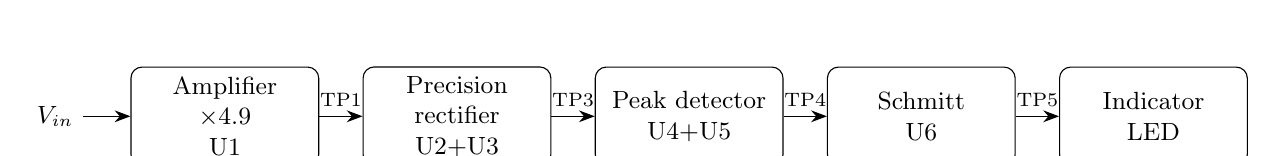
\begin{tikzpicture}[node distance=0.55cm, font=\small,
  blk/.style={draw, rounded corners, align=center, minimum height=1.25cm, text width=2.15cm},
  >={Stealth[length=2mm]}]
\node[blk] (a) {Amplifier\\$\times 4.9$\\U1};
\node[blk, right=of a] (b) {Precision rectifier\\U2+U3};
\node[blk, right=of b] (c) {Peak detector\\U4+U5};
\node[blk, right=of c] (d) {Schmitt\\U6};
\node[blk, right=of d] (e) {Indicator\\LED};
\draw[<-] (a.west) -- ++(-0.6,0) node[left]{$V_{in}$};
\draw[->] (a) -- node[above]{\scriptsize TP1} (b);
\draw[->] (b) -- node[above]{\scriptsize TP3} (c);
\draw[->] (c) -- node[above]{\scriptsize TP4} (d);
\draw[->] (d) -- node[above]{\scriptsize TP5} (e);
\end{tikzpicture}
\caption{Block diagram of the detector and test points.}\label{fig:bloques}
\end{figure}

\subsection{Schematic}

\begin{figure}[H]
\centering
\resizebox{\linewidth}{!}{% Complete schematic of the ECG heartbeat detector (circuitikz)
\begin{circuitikz}[european resistors, american inductors, font=\small]
\ctikzset{amplifiers/scale=0.75, diodes/scale=0.6, resistors/scale=0.7, capacitors/scale=0.7, grounds/scale=0.8}

% ================= ROW 1: amplifier + rectifier =================
% --- U1: non-inverting amplifier ---
\draw (0,0) node[ocirc]{} node[left]{$V_{in}$} to[short,-*] (1,0) coordinate(nin);
\node[op amp, noinv input up, anchor=+] (U1) at (2.4,0) {U1};
\draw (nin) -- (U1.+);
\draw (nin) to[R, l_={$R_0$\ 100\,k$\Omega$}] ++(0,-2.2) node[ground]{};
\draw (U1.-) -- ++(-0.35,0) coordinate(m1) -- (m1 |- 0,-2.0) coordinate(n1);
\coordinate (vg) at ($(U1.out)+(0.6,0)$);
\draw (U1.out) to[short,-*] (vg);
\draw (n1) to[R, l={$R_{g1}$\ 10\,k$\Omega$}, *-] ++(0,-1.6) node[ground]{};
\draw (n1) to[R, l={$R_{f1}$\ 39\,k$\Omega$}] (n1 -| vg) -- (vg);
\node[above] at (vg) {$V_g$ (TP1)};

% --- U2: inverting half-wave rectifier ---
\node[op amp, anchor=-] (U2) at ($(vg)+(3.6,0)$) {U2};
\coordinate (N) at ($(U2.-)+(-0.6,0)$);
\draw (vg) to[R, l={$R_2$\ 10\,k$\Omega$}, -*] (N) -- (U2.-);
\draw (U2.+) -- ++(-0.3,0) node[ground]{};
\coordinate (o2) at ($(U2.out)+(0.45,0)$);
\draw (U2.out) to[short,-*] (o2);
\draw (N) to[short,-*] (N |- 0,1.3) coordinate(d1l);
\draw (d1l -| o2) to[D, l_={$D_1$}] (d1l);
\draw (d1l -| o2) -- (o2);
\coordinate (vhwx) at ($(o2)+(1.3,0)$);
\draw (d1l) -- (N |- 0,2.6) to[R, l={$R_3$\ 10\,k$\Omega$}, -*] (vhwx |- 0,2.6) coordinate(VHW);
\draw (VHW) to[D, l={$D_2$}] (VHW |- o2) -- (o2);
\node[above right] at (VHW) {$V_{hw}$ (TP2)};

% --- U3: inverting summer ---
\coordinate (S) at ($(VHW)+(3.2,0)$);
\draw (VHW) to[R, l_={$R_5$\ 10\,k$\Omega$}, -*] (S);
\node[op amp, anchor=-] (U3) at ($(S |- 0,1.0)+(0.7,0)$) {U3};
\draw (S) -- (S |- U3.-) to[short,-] (U3.-);
\draw (U3.+) -- ++(-0.3,0) node[ground]{};
\coordinate (o3) at ($(U3.out)+(0.5,0)$);
\draw (U3.out) to[short,-*] (o3);
\draw (S) -- ++(0,1.2) coordinate(r6l) to[R, l={$R_6$\ 20\,k$\Omega$}] (r6l -| o3) -- (o3);
\draw (vg) to[short,*-] (vg |- 0,-4.0) to[R, l={$R_4$\ 20\,k$\Omega$}] (S |- 0,-4.0) to[short,-*] (S |- U3.-);
\node[above right] at (o3) {$V_r=|V_g|$ (TP3)};

% ================= ROW 2: peak detector + Schmitt + output =================
\coordinate (yrow) at (0,-8.0);
\draw (o3) -- ++(0.6,0) coordinate(o3b) -- (o3b |- 0,-5.6) -- (0.4,-5.6) coordinate(cr) -- (cr |- yrow) -- ++(1.0,0) coordinate(u4p);

% --- U4: detector ---
\node[op amp, noinv input up, anchor=+] (U4) at (u4p) {U4};
\coordinate (o4) at ($(U4.out)+(0.4,0)$);
\draw (U4.out) to[short,-*] (o4);
\draw (o4) to[D, l={$D_3$}] ++(1.6,0) to[R, l={$R_7$\ 100\,$\Omega$}] ++(2.0,0) coordinate(nc);
\draw (nc) to[C, l_={$C_1$\ 1\,$\mu$F}, *-] ++(0,-1.8) node[ground]{};
\draw (nc) to[short,-*] ++(1.4,0) coordinate(nc2);
\draw (nc2) to[R, l={$R_9$\ 100\,k$\Omega$}] ++(0,-1.8) node[ground]{};

% D4 and R8
\draw (U4.-) -- ++(-0.35,0) coordinate(a4) -- ++(0,-1.0) coordinate(d4l);
\draw (d4l) to[D, l_={$D_4$}, *-] (d4l -| o4) -- (o4);

% --- U5: buffer ---
\node[op amp, noinv input up, anchor=+] (U5) at ($(nc2)+(1.4,0)$) {U5};
\draw (nc2) -- (U5.+);
\coordinate (o5) at ($(U5.out)+(0.45,0)$);
\draw (U5.out) to[short,-*] (o5);
\draw (U5.-) -- ++(-0.3,0) -- ++(0,-0.9) -| (o5);
\coordinate (o6) at ($(o5)+(0.9,0)$);
\draw (o5) to[short,-*] (o6);
\node[above] at (o6) {$V_{env}$ (TP4)};
\draw (d4l) -- ++(0,-1.6) coordinate(r8l) to[R, l_={$R_8$\ 10\,k$\Omega$}] (r8l -| o6) -- (o6);

% --- U6: non-inverting Schmitt ---
\node[op amp, noinv input up, anchor=+] (U6) at ($(o6)+(3.0,0)$) {U6};
\coordinate (P) at ($(U6.+)+(-0.45,0)$);
\draw (o6) to[R, l_={$R_{10}$\ 10\,k$\Omega$}, -*] (P) -- (U6.+);
\coordinate (o7) at ($(U6.out)+(0.5,0)$);
\draw (U6.out) to[short,-*] (o7);
\draw (P) -- ++(0,1.3) coordinate(r11l) to[R, l={$R_{11}$\ 430\,k$\Omega$}] (r11l -| o7) -- (o7);
\draw (U6.-) -- ++(-0.45,0) coordinate(q0) -- ++(0,-1.1) coordinate(Q);
\draw (Q) to[R, l={$R_{13}$\ 1\,k$\Omega$}, *-] ++(0,-1.6) node[ground]{};
\draw (Q) to[R, l_={$R_{12}$\ 15\,k$\Omega$}] ++(-1.8,0) node[left]{$+12$\,V};
\node[right] at ($(Q)+(0.05,0.25)$) {\footnotesize $V_{ref}=0.75$\,V};

% --- Output ---
\draw (o7) to[D, l={$D_5$}] ++(1.5,0) coordinate(l1) to[R, l={$R_{14}$\ 1\,k$\Omega$}] ++(0,-1.8) to[led, l={LED}] ++(0,-1.5) node[ground]{};
\node[above] at (o7) {TP5};
\end{circuitikz}
}
\caption{Complete schematic. The $\pm\SI{12}{V}$ supply and the \SI{100}{nF} decoupling capacitors are not drawn.}\label{fig:esquema}
\end{figure}

The signal runs along the first row from left to right and moves to the second row at TP3. The connections of each op-amp are:
\begin{enumerate}
  \item \textbf{U1 (amplifier):} $(+)\leftarrow$ input, with R0 to ground; $(-)\leftarrow$ Rg1 to ground and Rf1 from the output. Output $=\Vg$ (TP1).
  \item \textbf{U2 (half-wave):} $(+)$ to ground; $(-)\leftarrow\Vg$ through R2. D1: anode at the U2 output, cathode at $(-)$. D2: cathode at the U2 output, anode at node $V_{hw}$. R3 from $(-)$ to $V_{hw}$ (TP2).
  \item \textbf{U3 (summer):} $(+)$ to ground; $(-)\leftarrow\Vg$ through R4 and $\leftarrow V_{hw}$ through R5; R6 from $(-)$ to the output. Output $=\Vr=|\Vg|$ (TP3).
  \item \textbf{U4 (detector):} $(+)\leftarrow\Vr$. Output $\rightarrow$ D3 $\rightarrow$ R7 $\rightarrow$ C1 node (C1 and R9 in parallel to ground). $(-)\leftarrow\Venv$ through R8. D4: anode at $(-)$, cathode at the U4 output.
  \item \textbf{U5 (buffer):} follower; $(+)\leftarrow$ C1 node, $(-)$ tied to the output. Output $=\Venv$ (TP4).
  \item \textbf{U6 (Schmitt):} $(+)\leftarrow\Venv$ through R10 and $\leftarrow$ U6 output through R11. $(-)\leftarrow\Vref$ (divider: R12 from $+\SI{12}{V}$, R13 to ground). Output $=$ TP5.
  \item \textbf{Indicator:} TP5 $\rightarrow$ D5 $\rightarrow$ R14 $\rightarrow$ LED $\rightarrow$ ground.
\end{enumerate}

% ---------------- Stage 1 ----------------
\subsection{Stage 1: non-inverting amplifier (U1)}

This is the first stage to be designed: it brings the input signal to a comfortable level for the rest of the circuit, moving it away from noise and offsets without reaching saturation.

\paragraph{Derivation.} The non-inverting input is connected to the signal, so $V_+=V_{in}$. The inverting input takes a fraction of the output through the Rf1--Rg1 divider:
\begin{equation}
V_- = \Vg\,\frac{R_{g1}}{R_{g1}+R_{f1}}
\end{equation}
Setting $V_-=V_+=V_{in}$ and solving:
\begin{equation}
\Vg = V_{in}\left(1+\frac{R_{f1}}{R_{g1}}\right) = V_{in}\left(1+\frac{\SI{39}{k\ohm}}{\SI{10}{k\ohm}}\right) = 4.9\,V_{in}
\label{eq:ganancia}
\end{equation}

\paragraph{Choice of gain.} At the start of the design only the input (peaks of 0.5 to \SI{2}{V}) and the op-amp saturation ($\Vsat\approx\SI{10.5}{V}$) are known; the comparator thresholds do not exist yet. The input varies over a 4:1 ratio, so it is not possible to place both the large and the small signal at an ideal level at the same time. The criterion is to \textbf{amplify as much as possible without saturating the largest signal}, so that the smallest one ends up as far as possible from noise and offsets.

\begin{enumerate}
  \item \textbf{Saturation limit.} The maximum input is the \SI{2}{V_{pp}} pulse with its low level at \SI{0}{V}, whose peak is \SI{2}{V}:
  \begin{equation}
  G\cdot\SI{2}{V}\le\Vsat\;\Rightarrow\;G_{max}=\frac{10.5}{2}=5.25
  \end{equation}
  Above this value the pulse is clipped and the peak detector no longer sees the real amplitude.
  \item \textbf{Standard value.} With $R_{g1}=\SI{10}{k\ohm}$, $R_{f1}=(G-1)R_{g1}\le\SI{42.5}{k\ohm}$. In the E12 series:
  \begin{itemize}
    \item $R_{f1}=\SI{39}{k\ohm}\Rightarrow G=4.9$, \SI{7}{\percent} below saturation.
    \item $R_{f1}=\SI{47}{k\ohm}\Rightarrow G=5.7$, which saturates.
  \end{itemize}
  $G=4.9$ is chosen, the largest standard gain that does not saturate.
  \item \textbf{Resulting range.} The amplified signal has peaks of
  \begin{equation}
  V_{p,min}=4.9\cdot0.5=\SI{2.45}{V},\qquad V_{p,max}=4.9\cdot2=\SI{9.8}{V}
  \end{equation}
  These values are the starting data for the following stages.
  \item \textbf{Requirement passed on to the comparator.} To detect the smallest signal with a margin of 2 against noise and tolerances, the Schmitt trigger threshold must satisfy
  \begin{equation}
  \VTH\le\frac{V_{p,min}}{2}=\frac{2.45}{2}=\SI{1.22}{V}
  \label{eq:vthmax}
  \end{equation}
  This condition is used in stage 4.
\end{enumerate}

Figure~\ref{fig:calcgan} shows the hand-worked reasoning behind this criterion: the saturation limit ($G\le5.25$), the choice of $G=4.9$ with margin, and the check of the maximum (\SI{9.8}{V}) and minimum (\SI{2.45}{V}) peaks against $\Vsat$.

\begin{figure}[H]
\centering
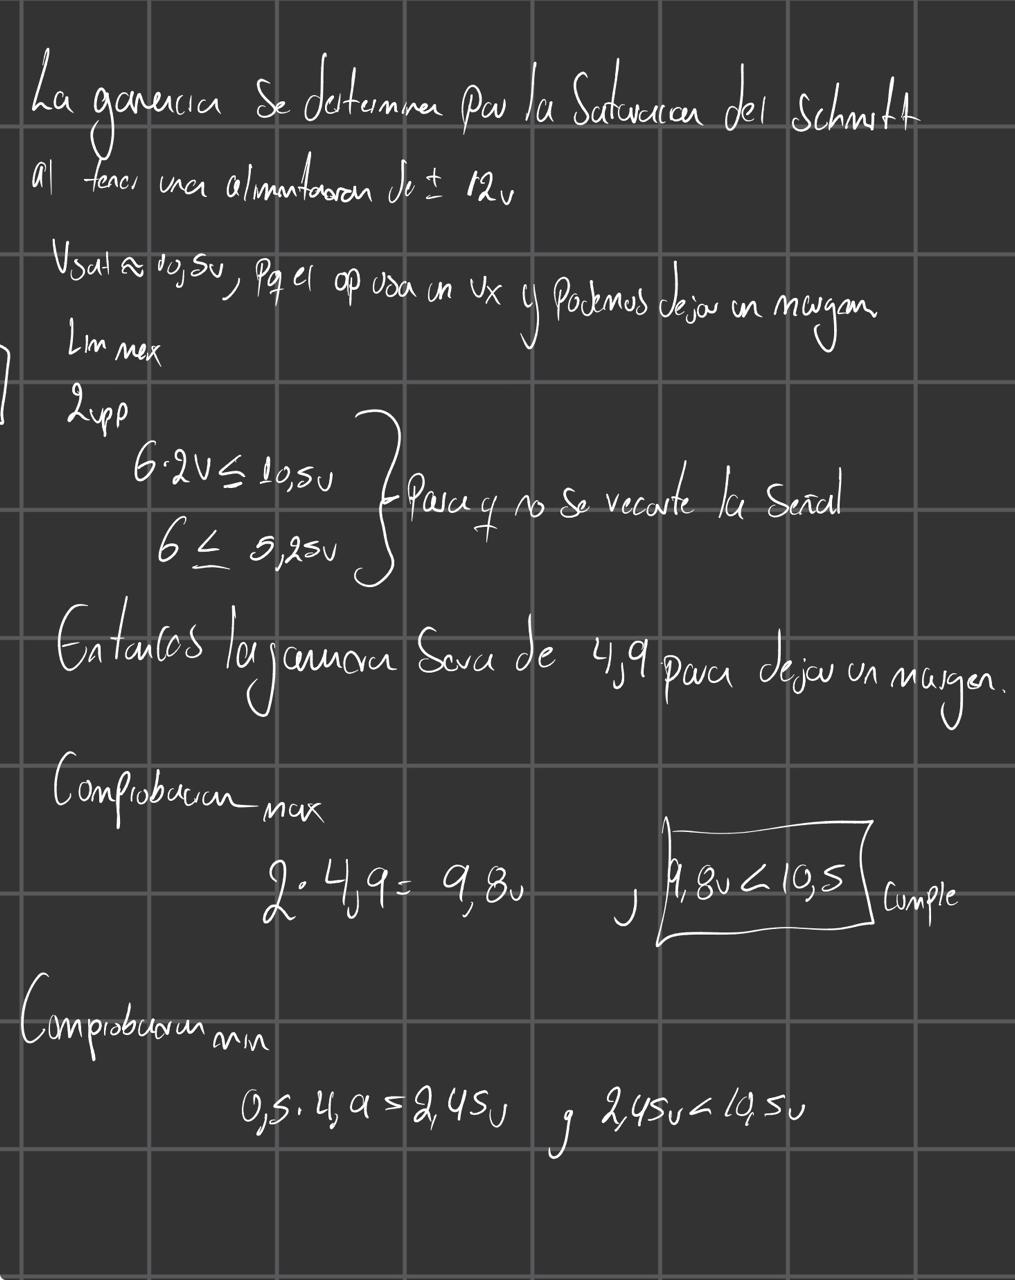
\includegraphics[width=0.62\linewidth]{calc_ganancia.png}
\caption{Hand calculation: choice of the non-inverting amplifier gain from saturation (handwritten, in Spanish).}\label{fig:calcgan}
\end{figure}

\paragraph{Verification.} With the Schmitt already designed ($\VTH=\SI{1.01}{V}$, stage 4), we check that the gain falls within the window imposed by both stages:
\begin{equation}
\underbrace{\frac{2\cdot1.01}{0.5}}_{4.04}\;\le\;G=4.9\;\le\;\underbrace{\frac{10.5}{2}}_{5.25}
\end{equation}

\paragraph{Non-idealities.} With a finite open-loop gain,
\begin{equation}
G_{real}=\frac{G}{1+G/A_{ol}}=\frac{4.9}{1+4.9/\num{200000}}\approx 4.8999
\end{equation}
with an error of \SI{0.0025}{\percent}. The bandwidth is $f_{-3dB}=GBW/G$: \SI{612}{kHz} with the TL074 and \SI{204}{kHz} with the LM324. The 0 to \SI{9.8}{V} edge takes \SI{0.75}{\micro s} with the TL074 and \SI{20}{\micro s} with the LM324, negligible compared with \SI{75}{ms}. The generator (\SI{50}{\ohm}) sees R0 $=\SI{100}{k\ohm}$: the attenuation is 0.9995.

\paragraph{Hand calculations.} Figure~\ref{fig:calcamp} reproduces the calculation done by hand: with $R_{g1}=\SI{10}{k\ohm}$ and $A_v=4.9$, solving gives $R_{f1}=(A_v-1)R_{g1}=\SI{39}{k\ohm}$.

\begin{figure}[H]
\centering
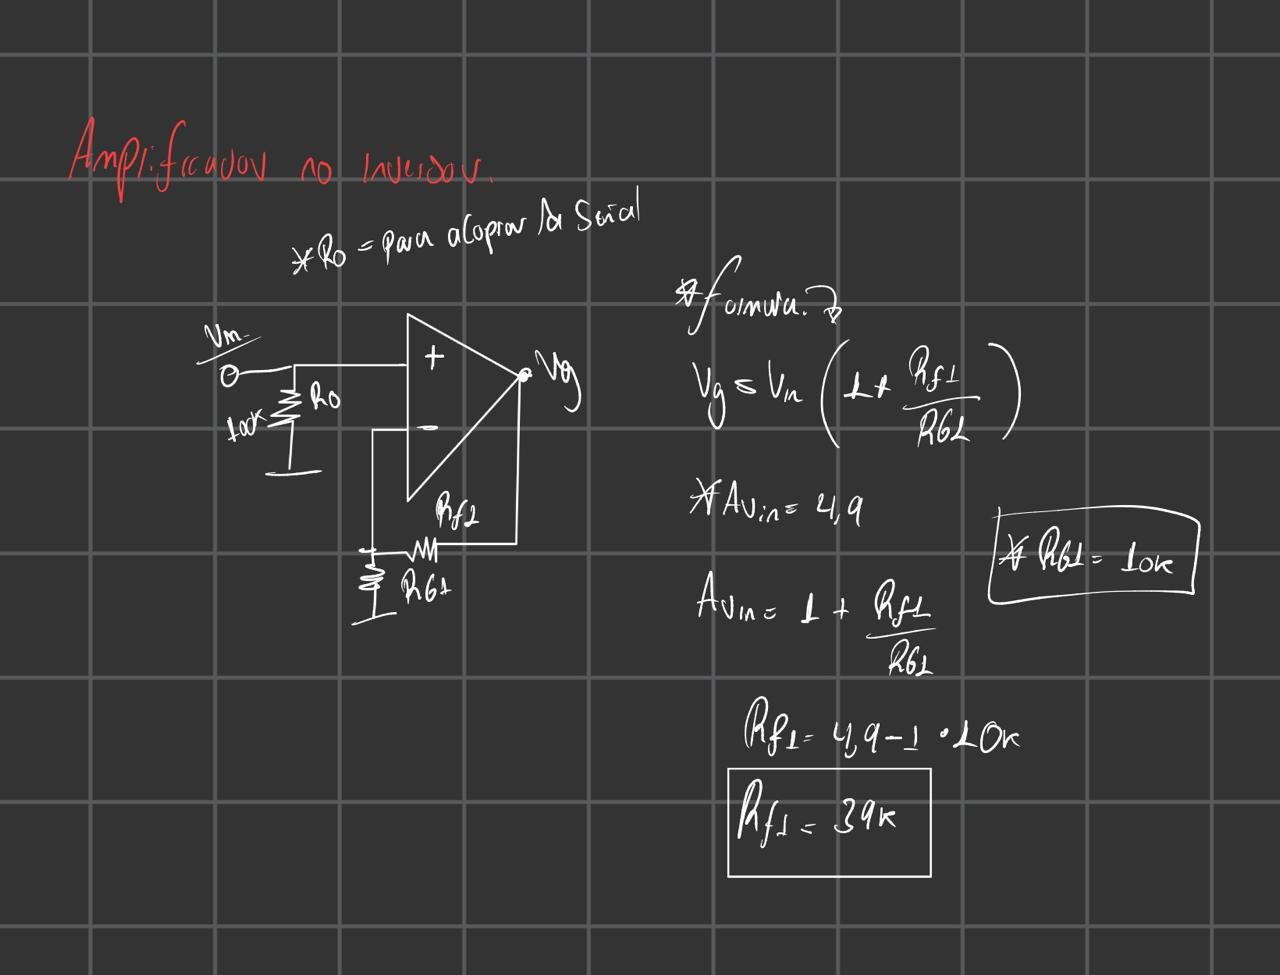
\includegraphics[width=\linewidth]{calc_amplificador.png}
\caption{Hand calculations: non-inverting amplifier (U1) (handwritten, in Spanish).}\label{fig:calcamp}
\end{figure}

% ---------------- Stage 2 ----------------
\subsection{Stage 2: full-wave precision rectifier (U2 + U3)}

This stage delivers $\Vr=|\Vg|$ with unity gain for both polarities.

\paragraph{Positive half-cycle ($\Vg>0$).} The $(+)$ input of U2 is grounded, so its $(-)$ input is a virtual ground. A current $i=\Vg/R_2$ enters through R2; since it cannot flow into the op-amp, it continues through R3 toward node $V_{hw}$. The U2 output goes down, D2 conducts and D1 is reverse-biased. Applying the current law at the inverting input:
\begin{equation}
\frac{\Vg-0}{R_2}=\frac{0-V_{hw}}{R_3}\;\Rightarrow\; V_{hw}=-\frac{R_3}{R_2}\Vg=-\Vg
\end{equation}
The U2 output sits one diode drop below: $V_{hw}-\SI{0.6}{V}$. That drop does not appear at $V_{hw}$ because the signal is taken after D2, inside the loop.

\paragraph{Negative half-cycle ($\Vg<0$).} The current through R2 leaves the node; the U2 output rises until D1 conducts and settles at $\approx+\SI{0.6}{V}$, almost independent of $\Vg$. D2 is reverse-biased, no current flows through R3 and R5, and $V_{hw}=0$.

\paragraph{Summer (U3).} With a virtual ground at its $(-)$ input, the current through R6 is the sum of the currents arriving through R4 and R5:
\begin{equation}
\frac{\Vg}{R_4}+\frac{V_{hw}}{R_5}=-\frac{\Vr}{R_6}\;\Rightarrow\;\Vr=-\left(\frac{R_6}{R_4}\Vg+\frac{R_6}{R_5}V_{hw}\right)=-\left(\Vg+2V_{hw}\right)
\label{eq:sumador}
\end{equation}
Substituting each half-cycle:
\begin{equation}
\Vg>0:\;\Vr=-(\Vg-2\Vg)=+\Vg \qquad \Vg<0:\;\Vr=-(\Vg+0)=-\Vg
\end{equation}
In both cases $\Vr=|\Vg|$. The path through R4 carries the full signal (before the rectifier) with weight 1; the path through R5 carries the half-wave signal with weight 2, which in the positive half-cycle cancels the wrong-sign term and adds it back with the correct sign.

\begin{table}[H]
\centering
\caption{Voltages and diode states with $\Vg=\pm\SI{4}{V}$.}\label{tab:rect4}
\begin{tabular}{@{}lcc@{}}
\toprule
 & $\Vg=+\SI{4}{V}$ & $\Vg=-\SI{4}{V}$ \\
\midrule
U2 output & $-\SI{4.6}{V}$ & $\approx+\SI{0.62}{V}$ \\
D1 / D2 & Off / on & On / off \\
$V_{hw}$ (TP2) & $-\SI{4}{V}$ & \SI{0}{V} \\
Current through D2 & \SI{0.8}{mA} (R3 + R5) & 0 \\
$\Vr$ (TP3) & $+\SI{4}{V}$ & $+\SI{4}{V}$ \\
\bottomrule
\end{tabular}
\end{table}

\begin{figure}[H]
\centering
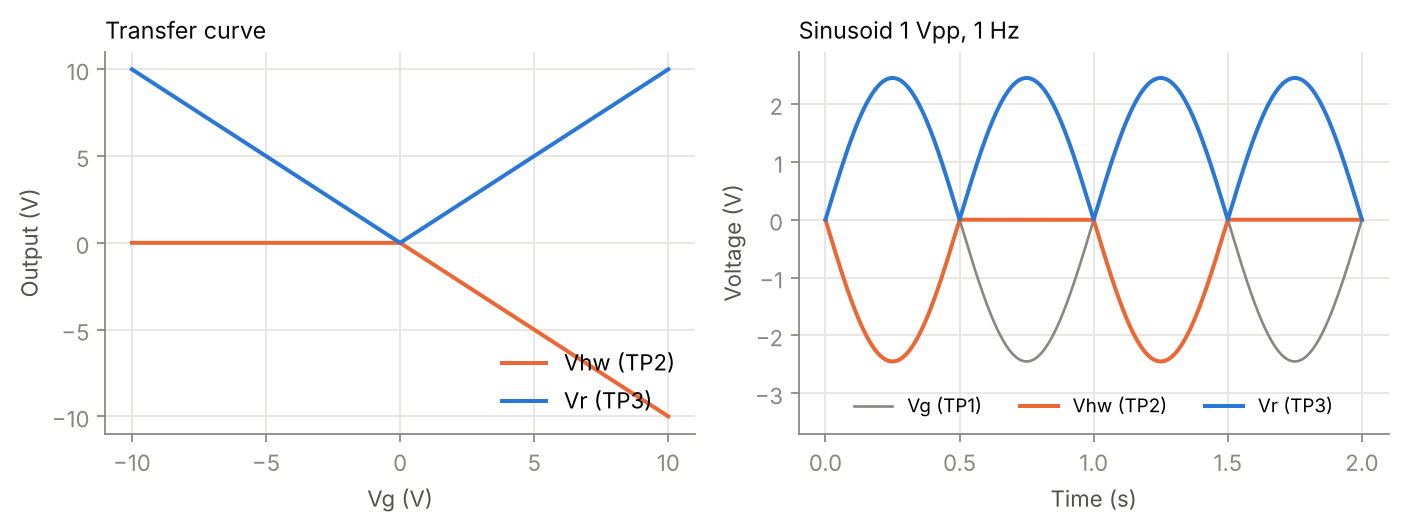
\includegraphics[width=\linewidth]{f1_rectificador.png}
\caption{Rectifier: transfer curve (left) and waveforms with a sine wave (right).}\label{fig:rect}
\end{figure}

\paragraph{Dead zone and transition.} For the diode to conduct, an input difference of only
\begin{equation}
V_{dead\,zone}=\frac{V_D}{A_{ol}}=\frac{\SI{0.6}{V}}{\num{200000}}=\SI{3}{\micro V}
\end{equation}
is needed. D1 keeps U2 from saturating: without it, in the negative half-cycle the loop would be open and the output would rise to $+\SI{10.5}{V}$. With D1 the output only jumps \SI{1.2}{V} at each zero crossing, which takes \SI{0.09}{\micro s} with the TL074 and \SI{2.4}{\micro s} with the LM324.

\paragraph{Sensitivity to tolerances.} Without assuming equal resistors:
\begin{equation}
G_+=\frac{R_6}{R_5}\cdot\frac{R_3}{R_2}-\frac{R_6}{R_4},\qquad G_-=\frac{R_6}{R_4}
\end{equation}
$G_+$ is the subtraction $2-1$, which carries the full error of each term. Evaluating the 32 combinations of $\pm$tolerance and a Monte Carlo simulation of \num{20000} circuits:

\begin{table}[H]
\centering
\caption{Difference between the gains of each half-cycle versus tolerance.}\label{tab:tol}
\begin{tabular}{@{}lcc@{}}
\toprule
Resistors & Worst case $|G_+-G_-|/G_-$ & 95th percentile \\
\midrule
\SI{1}{\percent} & \SI{8.2}{\percent} & \SI{2.6}{\percent} \\
\SI{5}{\percent} & \SI{44}{\percent} & \SI{13}{\percent} \\
\bottomrule
\end{tabular}
\end{table}

\paragraph{Hand calculations.} Figures~\ref{fig:calcrect} and~\ref{fig:calcsum} show the hand analysis of the half-wave rectifier in each half-cycle (with the example $\Vg=\pm\SI{4}{V}$) and of the summer, from which the conditions $R_3=R_2$, $R_6=R_4$ and $R_6=2R_5$ follow.

\begin{figure}[H]
\centering
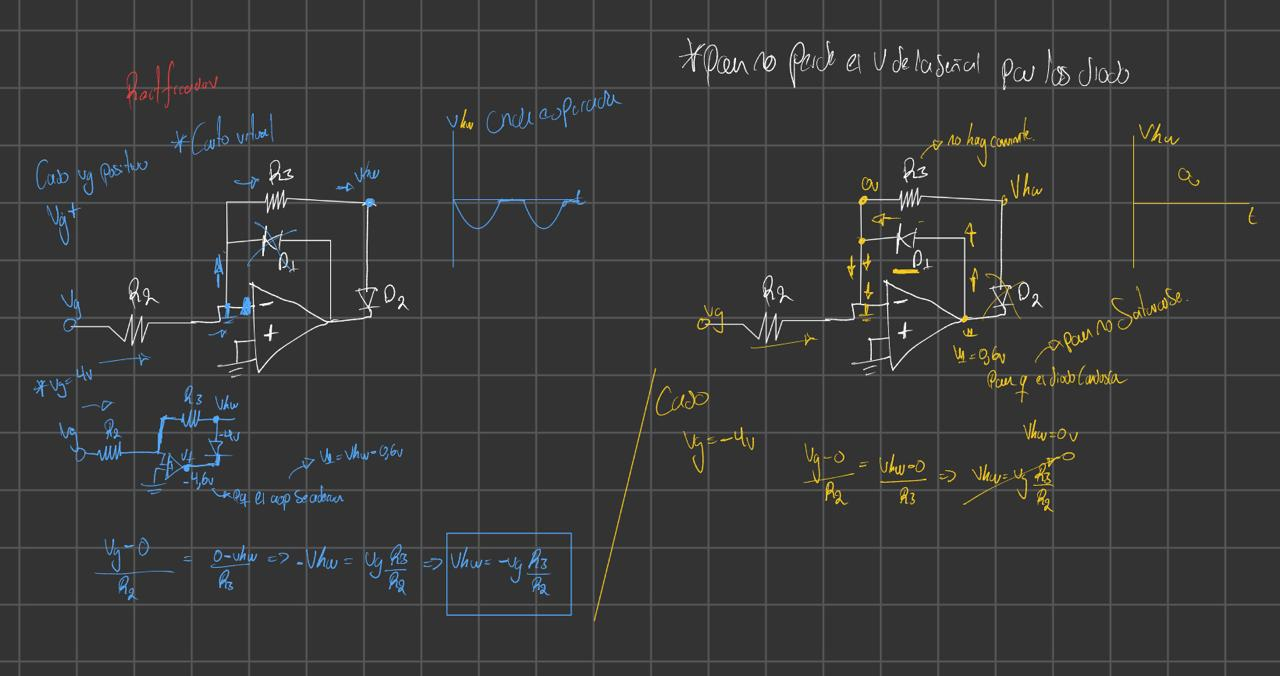
\includegraphics[width=\linewidth]{calc_rectificador.png}
\caption{Hand calculations: half-wave rectifier (U2) with positive and negative $\Vg$ (handwritten, in Spanish).}\label{fig:calcrect}
\end{figure}

\begin{figure}[H]
\centering
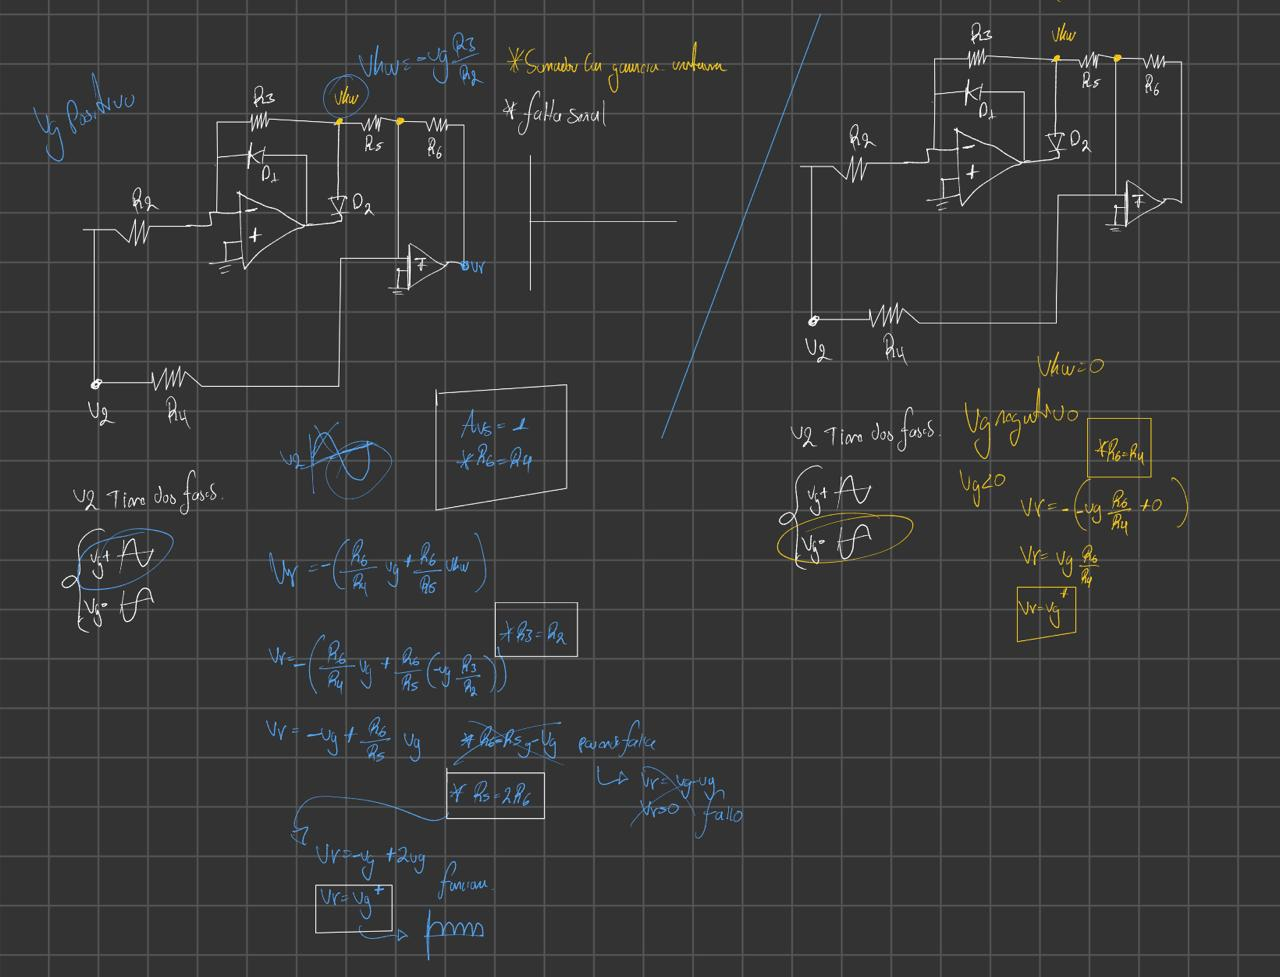
\includegraphics[width=\linewidth]{calc_sumador.png}
\caption{Hand calculations: inverting summer (U3) and conditions on R4, R5 and R6 (handwritten, in Spanish).}\label{fig:calcsum}
\end{figure}

% ---------------- Stage 3 ----------------
\subsection{Stage 3: peak detector (U4 + U5, C1, R9)}

The detector follows the rise of $\Vr$ in less than \SI{1}{ms}, holds it for the duration of the pulse and then discharges C1 with $\tau=\SI{100}{ms}$.

\begin{table}[H]
\centering
\caption{Starting data for the peak detector.}\label{tab:datos3}
\begin{tabularx}{\linewidth}{@{}llX@{}}
\toprule
Item & Value & Source \\
\midrule
Peak of $\Vr$ & 2.45 to \SI{9.8}{V} & Input of 0.5 to \SI{2}{V_{pp}} times the gain of 4.9 \\
Pulse width ($w$) & \SI{75}{ms} & Test pulse, similar to a QRS \\
Spacing between QRS lobes & $\approx\SI{20}{ms}$ & Typical time between the R and S waves \\
Maximum droop between lobes & \SI{20}{\percent} & Design criterion \\
Maximum heart rate & 150 bpm ($T=\SI{400}{ms}$) & Design range \\
Release threshold & $\VTL=\SI{0.52}{V}$ & Stage 4 \\
Maximum op-amp current & $\approx\SI{20}{mA}$ & Datasheet \\
Bias current & $\approx\SI{80}{nA}$ & 741 datasheet (worst case) \\
\bottomrule
\end{tabularx}
\end{table}

\subsubsection{Operation}

\paragraph{Charging ($\Vr>\Venv$).} U4 compares $\Vr$ ($+$ input) with $\Venv$, which reaches it through R8 from buffer U5 ($-$ input). If $\Vr$ is larger, the U4 output rises, D3 conducts and C1 charges through R7 until $\Venv=\Vr$. Since R8 takes the voltage after D3, the diode drop stays inside the loop: the U4 output settles $\approx\SI{0.5}{V}$ above $\Venv$ and $\Venv$ comes out equal to $\Vr$. Charging is limited by the maximum op-amp current:
\begin{equation}
\frac{d\Venv}{dt}=\frac{I_{max}}{C_1}=\frac{\SI{20}{mA}}{\SI{1}{\micro F}}=\SI{20}{V/ms}
\end{equation}
Reaching \SI{9.8}{V} takes $\approx\SI{0.5}{ms}$.

\paragraph{Discharging ($\Vr<\Venv$).} When the pulse ends, $\Vr$ drops to zero immediately, but C1 cannot change its voltage instantly. D3 is reverse-biased and the buffer input draws no current, so C1 discharges only through R9:
\begin{equation}
C_1\frac{d\Venv}{dt}=-\frac{\Venv}{R_9}\;\Rightarrow\;\Venv(t)=V_p\,e^{-t/\tau},\qquad \tau=R_9C_1
\label{eq:descarga}
\end{equation}
D4 closes the loop of U4: its $(-)$ input sits at $\Vr=0$ and its output at $\approx-\SI{0.6}{V}$, without saturating. The difference between $\Venv$ and that input appears across R8 (\SI{0.4}{mA} with $\Venv=\SI{4}{V}$), and that current is supplied by the buffer, not by C1.

\paragraph{Role of the buffer.} U5 is a follower ($V_{out}=V_{in}$, input impedance on the order of $10^{11}\,\Omega$). Without it, C1 would also discharge through R8 and $\tau$ would drop to $(R_9\parallel R_8)C_1\approx\SI{9}{ms}$; the envelope would fall between the QRS lobes and a single beat would produce several pulses.

\paragraph{Time to release the comparator.} From $V_p\,e^{-t/\tau}=\VTL$:
\begin{equation}
t_{desc}=\tau\,\ln\frac{V_p}{\VTL}
\label{eq:tdesc}
\end{equation}

\begin{table}[H]
\centering
\caption{Discharge time and output pulse width.}\label{tab:tdesc}
\begin{tabular}{@{}cccc@{}}
\toprule
Input & $V_p$ & $t_{desc}$ & Output width ($w+t_{desc}$) \\
\midrule
\SI{0.5}{V_{pp}} & \SI{2.45}{V} & \SI{154}{ms} & \SI{229}{ms} \\
\SI{1}{V_{pp}} & \SI{4.90}{V} & \SI{224}{ms} & \SI{299}{ms} \\
\SI{2}{V_{pp}} & \SI{9.80}{V} & \SI{293}{ms} & \SI{368}{ms} \\
\bottomrule
\end{tabular}
\end{table}

\begin{figure}[H]
\centering
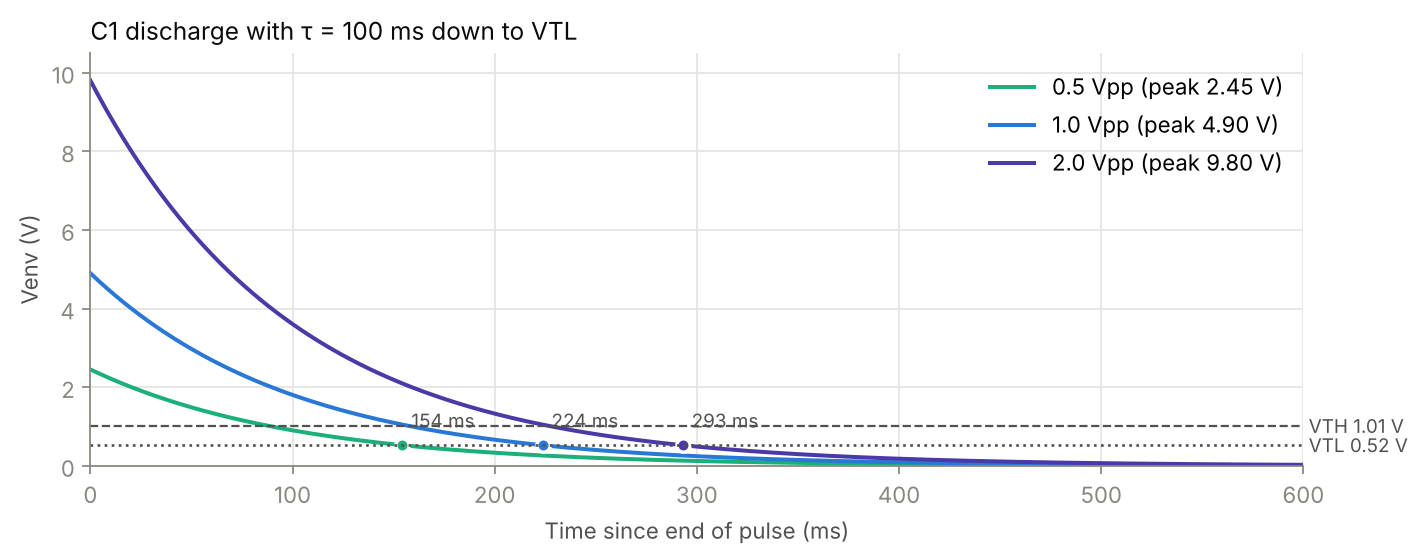
\includegraphics[width=\linewidth]{f3_descarga.png}
\caption{Discharge of C1 down to $\VTL$ for the three amplitudes.}\label{fig:descarga}
\end{figure}

\subsubsection{Component design}

\paragraph{Lower limit of $\tau$.} The QRS is not a single pulse: its lobes (Q, R and S) are about \SI{20}{ms} apart and the whole complex lasts 80 to \SI{120}{ms} in an adult~\cite{guyton}. Between lobes the envelope must not lose more than \SI{20}{\percent} (design criterion), so that the comparator is not released in the middle of the complex and does not count one beat twice:
\begin{equation}
e^{-\SI{20}{ms}/\tau}>0.8\;\Rightarrow\;\tau>\frac{\SI{20}{ms}}{\ln(1/0.8)}\approx\SI{90}{ms}
\end{equation}

\paragraph{Discharge condition.} The condition for the upper limit is derived by following one complete beat:
\begin{enumerate}
  \item \textbf{Charge.} The pulse arrives and C1 charges to the peak $V_p$ in $\approx\SI{0.1}{ms}$ ($R_7C_1$). $\Venv$ exceeds $\VTH$ and the Schmitt output goes high.
  \item \textbf{Hold.} For the duration of the pulse ($w$), U4 holds C1 at $V_p$.
  \item \textbf{Discharge.} When the pulse ends, D3 turns off and C1 discharges only through R9, following the natural response of an RC circuit~\cite{sedra,boylestad}: $\Venv(t)=V_p\,e^{-t/\tau}$.
  \item \textbf{Release.} The Schmitt returns low when $\Venv=\VTL$~\cite{sedra}, which happens after the discharge time $t_{desc}=\tau\ln(V_p/\VTL)$ of equation~\eqref{eq:tdesc}.
\end{enumerate}
From the start of one beat until the comparator is ready for the next one, $w+t_{desc}$ elapses. If the next beat arrives earlier, $\Venv$ is still above $\VTL$, the output does not go low and the two beats are counted as one. The condition for detecting each beat separately is therefore
\begin{equation}
w+\tau\ln\frac{V_p}{\VTL}<T=\frac{60}{HR}
\label{eq:condesc}
\end{equation}
This time plays the same role as the \emph{refractory period} of software QRS detectors, which ignore any event for about \SI{200}{ms} after each beat~\cite{pantompkins}. Here the refractory period is not programmed: it is set by $\tau$, $V_p$ and $\VTL$.

\paragraph{Upper limit of $\tau$.} The worst case is the highest peak (\SI{9.8}{V}, which takes longest to discharge) at the highest rate in the assignment (150 bpm, $T=\SI{400}{ms}$). With $\VTL=\SI{0.52}{V}$ (stage 4) in equation~\eqref{eq:condesc}:
\begin{equation}
\SI{75}{ms}+\tau\ln\frac{9.8}{0.52}<\SI{400}{ms}\;\Rightarrow\;\tau<\frac{\SI{325}{ms}}{2.94}\approx\SI{110}{ms}
\end{equation}

The midpoint of the \SIrange{90}{110}{ms} window is chosen, $\tau=\SI{100}{ms}$.

\paragraph{Maximum heart rate.} Solving equation~\eqref{eq:condesc} for $HR$ gives the maximum rate the circuit can count for any amplitude:
\begin{equation}
HR_{max}=\frac{60}{w+\tau\ln(V_p/\VTL)}\ \text{bpm}
\label{eq:fcmax}
\end{equation}

\begin{table}[H]
\centering
\caption{Maximum heart rate with $\tau=\SI{100}{ms}$, $w=\SI{75}{ms}$ and $\VTL=\SI{0.523}{V}$.}\label{tab:fcmax}
\begin{tabular}{@{}cccccc@{}}
\toprule
Input & $V_p$ & $V_p/\VTL$ & $t_{desc}=\tau\ln(V_p/\VTL)$ & $w+t_{desc}$ & $HR_{max}$ \\
\midrule
\SI{0.5}{V_{pp}} & \SI{2.45}{V} & 4.68 & \SI{154}{ms} & \SI{229}{ms} & 262 bpm \\
\SI{1}{V_{pp}} & \SI{4.9}{V} & 9.37 & \SI{224}{ms} & \SI{299}{ms} & 201 bpm \\
\SI{2}{V_{pp}} & \SI{9.8}{V} & 18.7 & \SI{293}{ms} & \SI{368}{ms} & 163 bpm \\
\bottomrule
\end{tabular}
\end{table}

Example with \SI{2}{V_{pp}}: $t_{desc}=0.1\ln(18.7)=\SI{0.293}{s}$, $w+t_{desc}=\SI{0.368}{s}$ and $HR_{max}=60/0.368=163$ bpm. The larger the peak, the longer C1 takes to fall to $\VTL$, which is why the maximum rate decreases with amplitude. In every case it stays above the 150 bpm required by the assignment.

\begin{figure}[H]
\centering
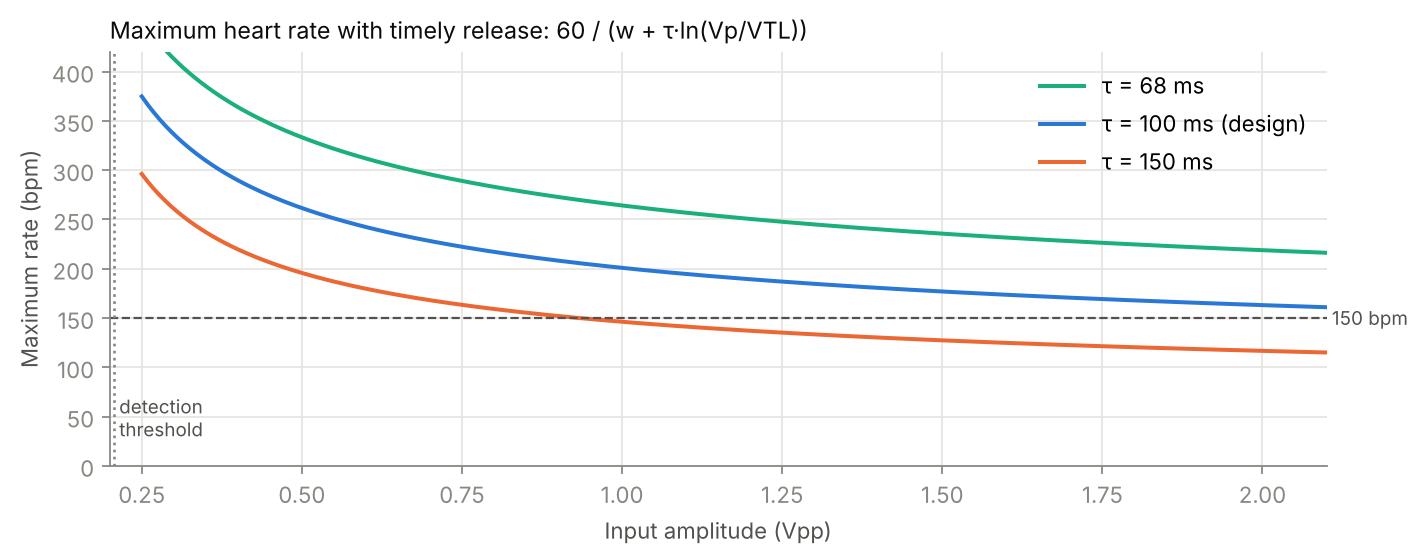
\includegraphics[width=\linewidth]{f4_fmax.png}
\caption{Maximum heart rate versus input amplitude for three values of $\tau$.}\label{fig:fmax}
\end{figure}

\paragraph{C1 and R9.} The \SI{100}{ms} product allows several combinations:

\begin{table}[H]
\centering
\caption{Options for obtaining $\tau=\SI{100}{ms}$.}\label{tab:c1r9}
\begin{tabularx}{\linewidth}{@{}llX@{}}
\toprule
C1 & R9 & Outcome \\
\midrule
\SI{10}{\micro F} & \SI{10}{k\ohm} & Rejected: an electrolytic has \si{\micro A} leakage and $\pm\SI{20}{\percent}$ tolerance \\
\SI{1}{\micro F} & \SI{100}{k\ohm} & Chosen: stable polyester; bias error $\SI{80}{nA}\times\SI{100}{k\ohm}=\SI{8}{mV}$ \\
\SI{100}{nF} & \SI{1}{M\ohm} & Rejected: bias error of \SI{80}{mV}, \SI{15}{\percent} of $\VTL$ \\
\bottomrule
\end{tabularx}
\end{table}

\paragraph{R7 and R8.} R7 must give a charge much faster than the rise of the QRS ($\tau_c=R_7C_1\le\SI{1}{ms}$, i.e.\ $R_7\le\SI{1}{k\ohm}$) and isolate the op-amp from the capacitive load (more than $\approx\SI{50}{\ohm}$); \SI{100}{\ohm} was chosen. During discharge, R8 carries $(\Venv-\Vr)/R_8$, at most \SI{0.98}{mA} with \SI{10}{k\ohm}; with M$\Omega$ resistors the bias current would create errors of tens of mV. Its useful range is \SI{1}{k\ohm} to \SI{100}{k\ohm}, and \SI{10}{k\ohm} was chosen.

\begin{table}[H]
\centering
\caption{Summary of the detector sizing.}\label{tab:res3}
\begin{tabular}{@{}llll@{}}
\toprule
Component & Governing condition & Valid range & Value \\
\midrule
$\tau=R_9C_1$ & Merge the QRS and release at 150 bpm & 90--\SI{110}{ms} & \SI{100}{ms} \\
C1 & Stable film & --- & \SI{1}{\micro F} \\
R9 & $\tau/C_1$ & --- & \SI{100}{k\ohm} \\
R7 & Fast charge and stability & \SI{100}{\ohm}--\SI{1}{k\ohm} & \SI{100}{\ohm} \\
R8 & Buffer current and bias & \SI{1}{k\ohm}--\SI{100}{k\ohm} & \SI{10}{k\ohm} \\
\bottomrule
\end{tabular}
\end{table}

\subsubsection{Behavior with a sine wave}
With $\Vr=A|\sin\omega t|$ the envelope follows the signal while the signal falls more slowly than the exponential, and separates from it when $\tan\varphi<\omega\tau$. At the zero crossing it is approximately
\begin{equation}
V_{env,min}\approx A\sin\varphi_0\,e^{-\varphi_0/(\omega\tau)},\qquad \varphi_0=\arctan(\omega\tau)
\end{equation}
With $A=\SI{4.9}{V}$: at \SI{0.5}{Hz}, $V_{env,min}\approx\SI{0.56}{V}$ (the simulation gives \SI{0.42}{V}) and two pulses per cycle are seen; at \SI{1}{Hz}, $V_{env,min}\approx\SI{1.07}{V}>\VTL$ and the comparator stays high. This is why the sine-wave test is done at \SI{0.5}{Hz}.

\paragraph{Hand calculations.} Figure~\ref{fig:calcdet} collects the hand analysis of charging and discharging, the equation for $\Venv(t)$ and the calculation of $C_1=\SI{1}{\micro F}$ and $R_9=\SI{100}{k\ohm}$.

\begin{figure}[H]
\centering
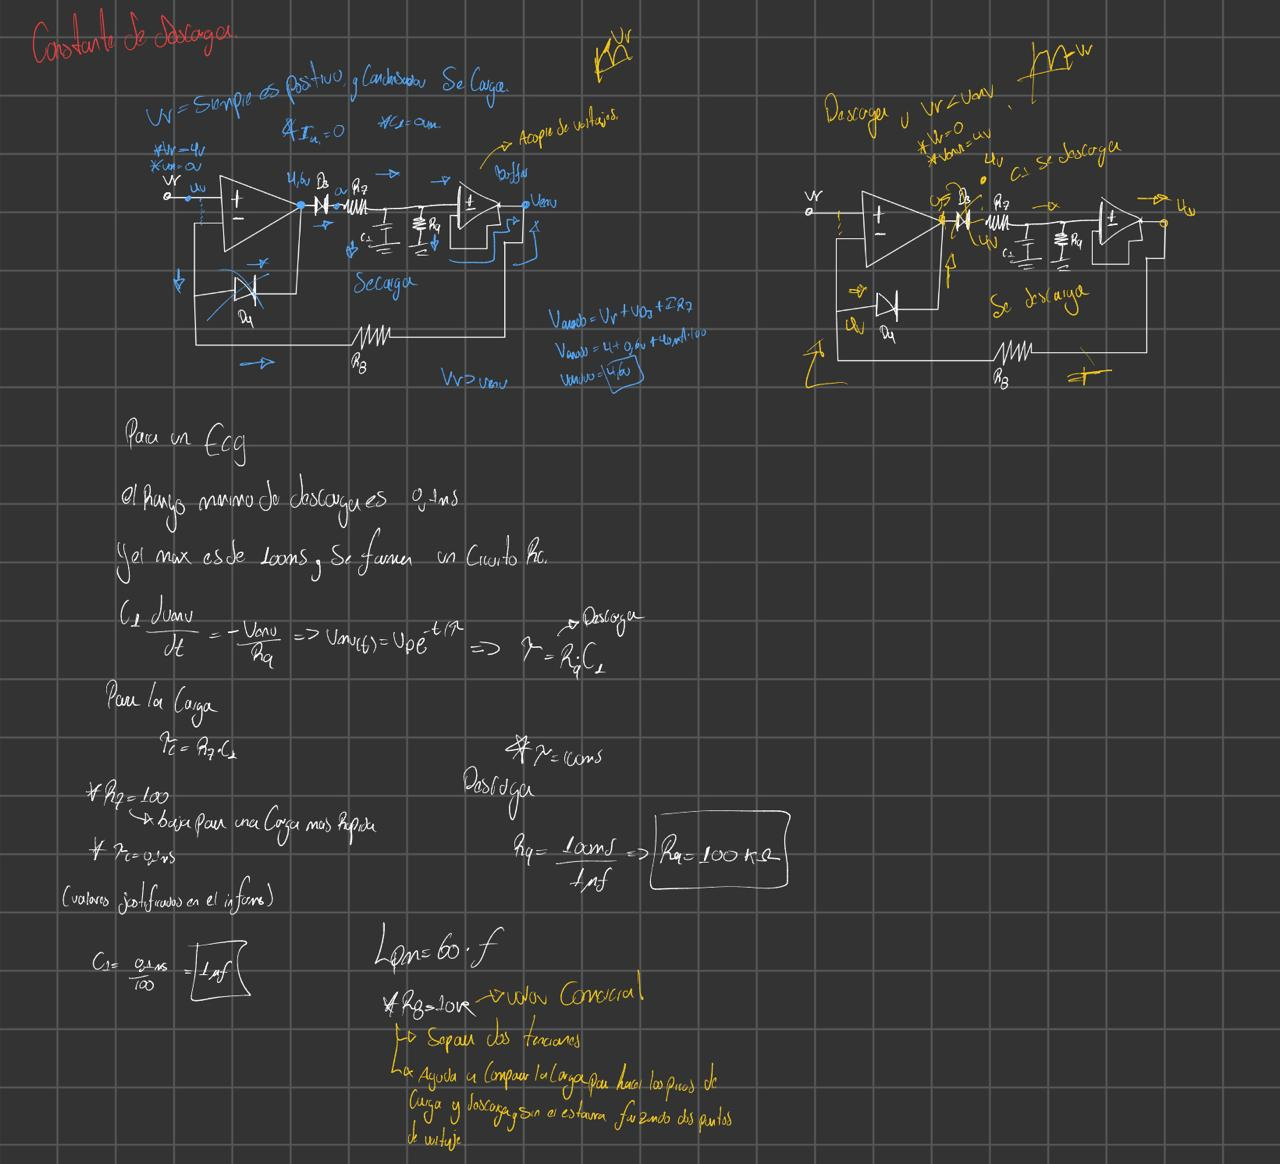
\includegraphics[width=\linewidth]{calc_detector.png}
\caption{Hand calculations: peak detector (U4, U5), charging, discharging and time constant (handwritten, in Spanish).}\label{fig:calcdet}
\end{figure}

% ---------------- Stage 4 ----------------
\subsection{Stage 4: non-inverting Schmitt comparator (U6)}

\paragraph{Choice of thresholds.} This stage is designed right after stage 1, because its thresholds depend on the minimum peak of the amplified signal ($V_{p,min}=\SI{2.45}{V}$) and stage 3 needs to know $\VTL$. The thresholds are chosen with margin relative to the signals:
\begin{itemize}
  \item $\VTH\approx\SI{1}{V}$, which meets condition~\eqref{eq:vthmax} ($\VTH\le\SI{1.22}{V}$): it is at half or less of the minimum pulse peak (\SI{2.45}{V}) and below the peak of the \SI{0.5}{V_{pp}} sine wave (\SI{1.22}{V}).
  \item $\VTL\approx\SI{0.5}{V}$, well above the accumulated offset on $\Venv$ (tens of mV) and below the T wave.
  \item $\Delta V\approx\SI{0.5}{V}$, about ten times the expected noise on the envelope.
\end{itemize}

\paragraph{Equations.} U6 has no negative feedback: its output is always at $\pm\Vsat$ and there is no virtual short. By superposition, with $k=R_{10}/R_{11}$:
\begin{equation}
V_+=\Venv\,\frac{R_{11}}{R_{10}+R_{11}}+V_o\,\frac{R_{10}}{R_{10}+R_{11}}
\end{equation}
The output switches when $V_+=\Vref$:
\begin{equation}
\Venv=\Vref(1+k)-V_o\,k
\end{equation}
With $V_o=-\Vsat$ (before the beat) and $V_o=+\Vsat$ (during the beat):
\begin{equation}
\VTH=\Vref(1+k)+\Vsat\,k,\qquad \VTL=\Vref(1+k)-\Vsat\,k
\end{equation}
\begin{equation}
\Delta V=\VTH-\VTL=2\Vsat\,k,\qquad V_c=\frac{\VTH+\VTL}{2}=\Vref(1+k)
\label{eq:hist}
\end{equation}

\paragraph{Sizing.}
\begin{enumerate}
  \item $k=\Delta V/(2\Vsat)=0.5/21=0.0238$. With $R_{10}=\SI{10}{k\ohm}$: $R_{11}=R_{10}/k=\SI{420}{k\ohm}\rightarrow\SI{430}{k\ohm}$ (E24), $k=0.02326$.
  \item $\Vref=V_c/(1+k)\approx\SI{0.75}{V}$. With the divider from $+\SI{12}{V}$: $R_{13}/(R_{12}+R_{13})=1/16$, i.e.\ $R_{12}=\SI{15}{k\ohm}$ and $R_{13}=\SI{1}{k\ohm}$.
\end{enumerate}
With the standard values:
\begin{equation}
\VTH=0.750(1.02326)+10.5(0.02326)=0.767+0.244=\SI{1.012}{V}
\end{equation}
\begin{equation}
\VTL=0.767-0.244=\SI{0.523}{V},\qquad \Delta V=\SI{0.488}{V}
\end{equation}

\begin{figure}[H]
\centering
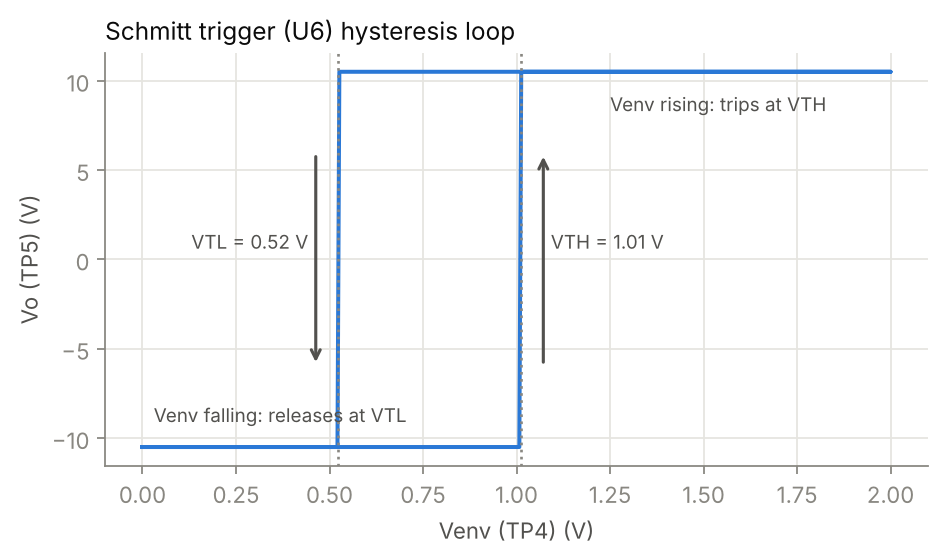
\includegraphics[width=0.7\linewidth]{f5_histeresis.png}
\caption{Hysteresis loop of the comparator: $V_o$ versus $\Venv$.}\label{fig:hist}
\end{figure}

\paragraph{Regenerative feedback.} When the comparator trips, the term $V_o\,k$ changes from $-\SI{0.244}{V}$ to $+\SI{0.244}{V}$ and $V_+$ jumps from \SI{0.75}{V} to \SI{1.228}{V}, far away from $\Vref$. This is why noise cannot switch the output back. The current through R11 and R10 (about \SI{15}{\micro A}) is supplied by buffer U5, so it does not disturb the discharge of C1.

\paragraph{Sensitivity.} A one-volt change in $\Vsat$ shifts each threshold by \SI{23}{mV}; a $\pm\SI{5}{\percent}$ error on the $+\SI{12}{V}$ rail shifts them by $\pm\SI{38}{mV}$.

\paragraph{Hand calculations.} Figure~\ref{fig:calcsch} shows the hand calculation of the thresholds, of $R_{11}$ from the hysteresis, of the $R_{12}$--$R_{13}$ divider, and the check of $\VTH$ and $\VTL$.

\begin{figure}[H]
\centering
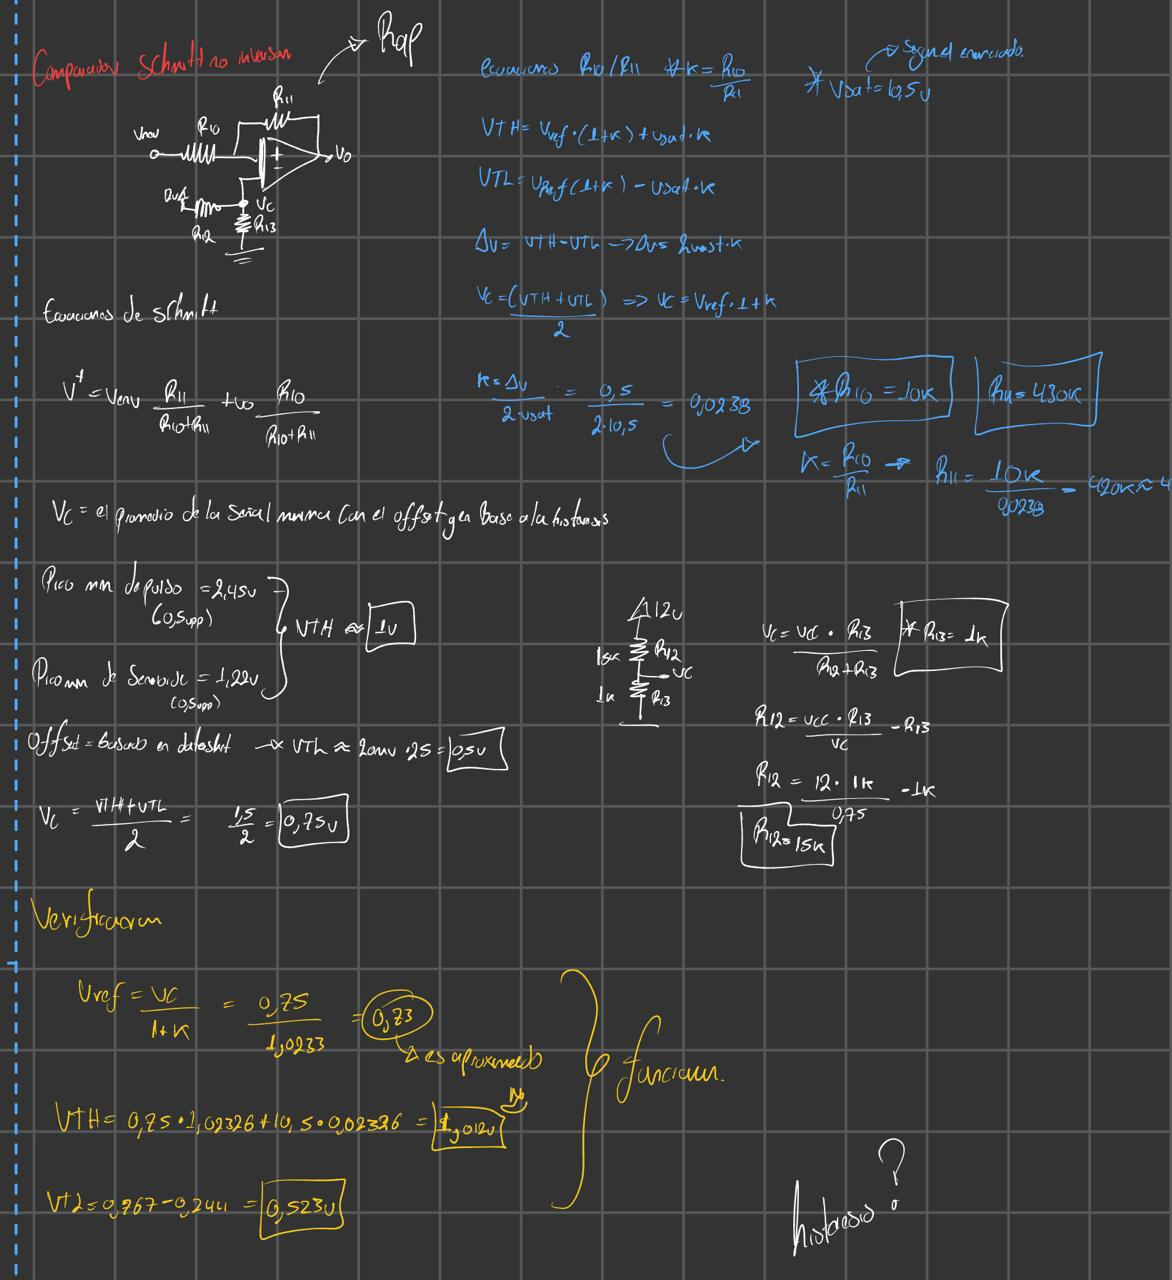
\includegraphics[width=0.88\linewidth]{calc_schmitt.png}
\caption{Hand calculations: non-inverting Schmitt comparator (U6) and reference divider (handwritten, in Spanish).}\label{fig:calcsch}
\end{figure}

% ---------------- Stage 5 ----------------
\subsection{Stage 5: LED indicator}

With $V_o=+\SI{10.5}{V}$, D5 and the LED conduct:
\begin{equation}
I_{LED}=\frac{\Vsat-V_{D5}-V_{LED}}{R_{14}}=\frac{10.5-0.7-2.0}{\SI{1}{k\ohm}}=\SI{7.8}{mA}
\end{equation}
The D5 drop (\SI{0.7}{V}) is that of a silicon diode at mA-level current, and the drop of the red LED (\SI{2}{V}) is taken from its datasheet. With $V_o=-\SI{10.5}{V}$, D5 blocks the reverse voltage (the 1N4148 withstands \SI{100}{V}) and protects the LED, which only tolerates about \SI{5}{V} in reverse.

A blue LED was used in the build, with a drop of about \SI{3}{V}; with the measured high level of \SI{11.1}{V} the current is $(11.1-0.7-3.0)/\SI{1}{k\ohm}\approx\SI{7.4}{mA}$, practically the same as in the design.

The heart rate is obtained by counting the rising edges at TP5: $HR = 60/T_{RR}$, where $T_{RR}$ is the time between two edges.

% ---------------------------- 6. SIMULATION --------------------------
\section{Simulation}

\subsection{Behavioral simulation (Python)}

Each stage was coded with the equations of the previous section at \num{20000} samples per second (code in Appendix~\ref{anx:codigo}): a gain of 4.9 with clipping at $\pm\SI{10.5}{V}$, ideal rectification, charging with $\tau_c=\SI{0.1}{ms}$ and exponential discharge with $\tau=\SI{100}{ms}$, and a comparator with state. It does not include slew rate or diode drops, which at these frequencies account for less than \SI{1}{\percent}.

\begin{figure}[H]
\centering
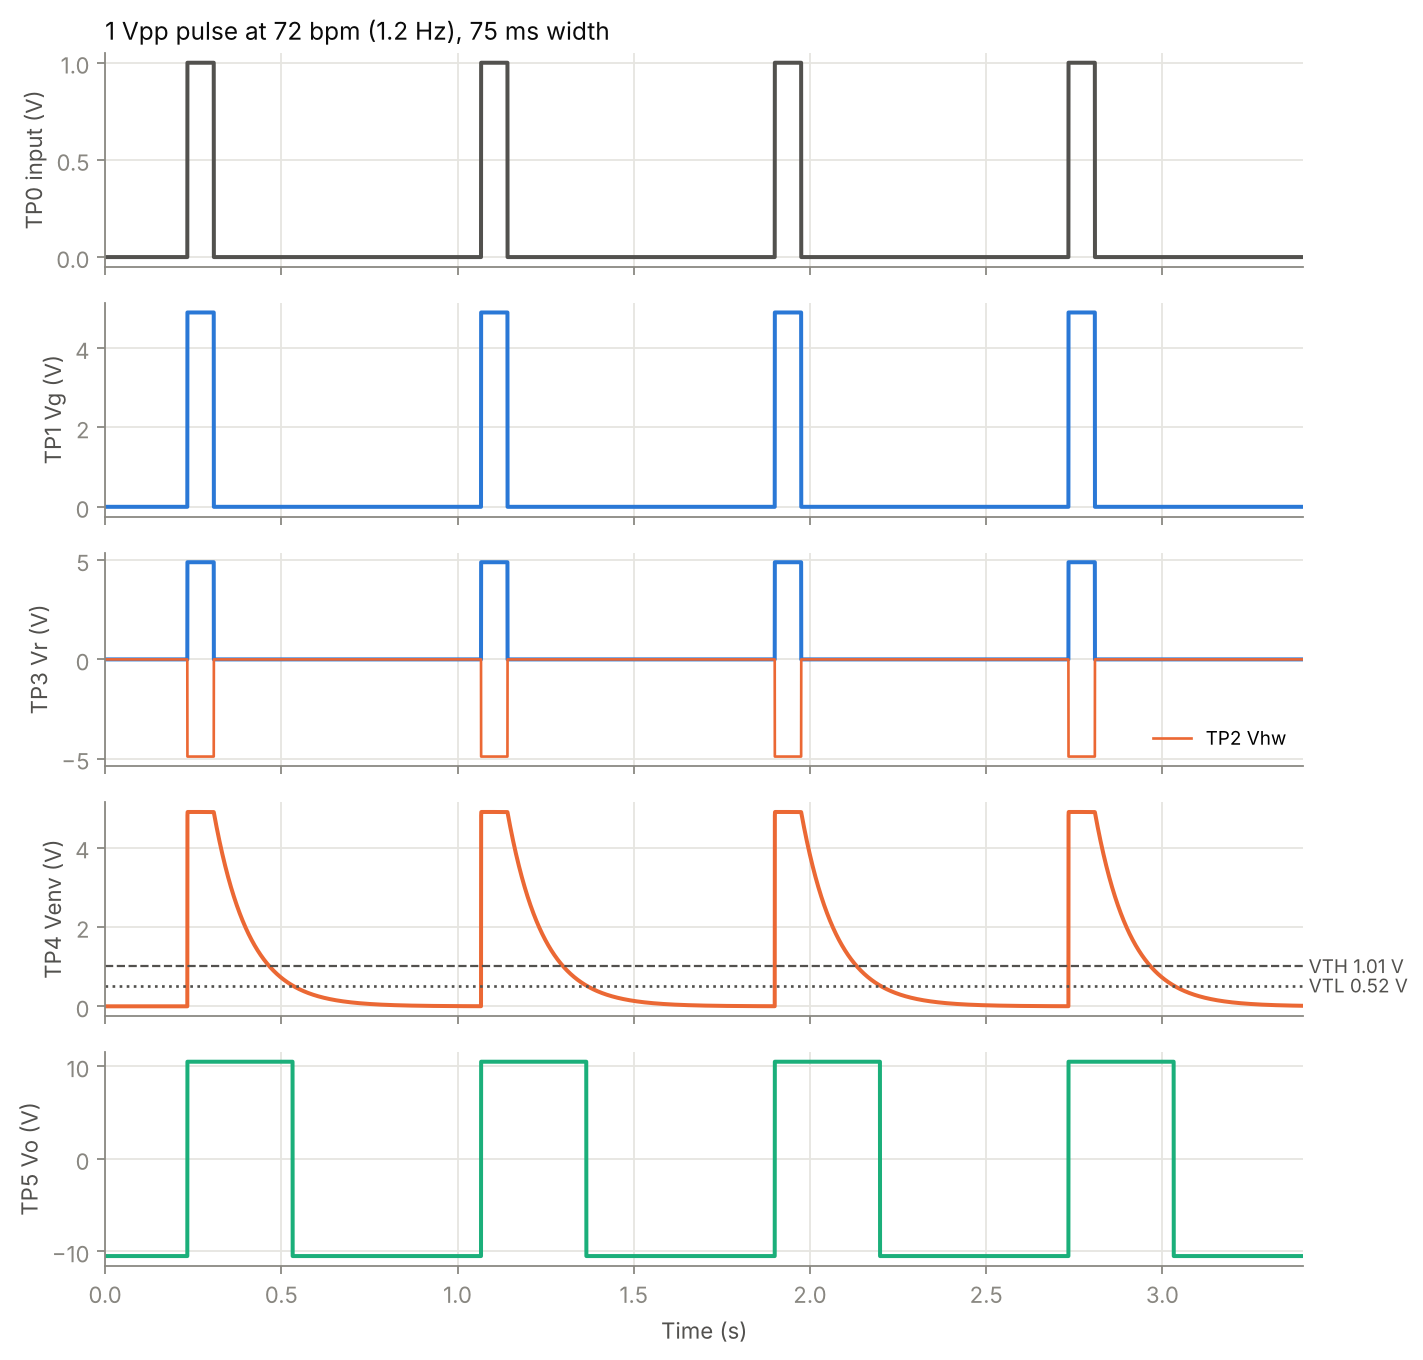
\includegraphics[width=0.95\linewidth]{f2_pulso_72lpm.png}
\caption{Waveforms at TP0 to TP5 with a \SI{1}{V_{pp}} pulse at 72 bpm.}\label{fig:pulso}
\end{figure}

{\small\setlength{\tabcolsep}{4pt}
\begin{longtable}{@{}ccccccc@{}}
\caption{Rate and amplitude sweep with a pulse (positive and negative polarity gave identical results).}\label{tab:barrido}\\
\toprule
HR (bpm) & Input (V$_{pp}$) & Beats & Detected & Width (ms) & $\Venv$ peak (V) & $\Venv$ before (V) \\
\midrule
\endfirsthead
\toprule
HR (bpm) & Input (V$_{pp}$) & Beats & Detected & Width (ms) & $\Venv$ peak (V) & $\Venv$ before (V) \\
\midrule
\endhead
40 & 0.5 & 6 & 6 & 229 & 2.45 & 0.00 \\
40 & 1.0 & 6 & 6 & 299 & 4.90 & 0.00 \\
40 & 2.0 & 6 & 6 & 368 & 9.79 & 0.00 \\
72 & 0.5 & 12 & 12 & 229 & 2.45 & 0.00 \\
72 & 1.0 & 12 & 12 & 299 & 4.90 & 0.00 \\
72 & 2.0 & 12 & 12 & 368 & 9.79 & 0.00 \\
120 & 0.5 & 20 & 20 & 229 & 2.45 & 0.03 \\
120 & 1.0 & 20 & 20 & 299 & 4.90 & 0.07 \\
120 & 2.0 & 20 & 20 & 368 & 9.79 & 0.14 \\
150 & 0.5 & 25 & 25 & 229 & 2.45 & 0.09 \\
150 & 1.0 & 25 & 25 & 299 & 4.90 & 0.19 \\
150 & 2.0 & 25 & 25 & 368 & 9.79 & 0.38 \\
180 & 0.5 & 30 & 30 & 229 & 2.45 & 0.18 \\
180 & 1.0 & 30 & 30 & 299 & 4.90 & 0.37 \\
180 & 2.0 & 30 & 1 (stuck high) & --- & 9.79 & 0.74 \\
\bottomrule
\end{longtable}
}

\begin{figure}[H]
\centering
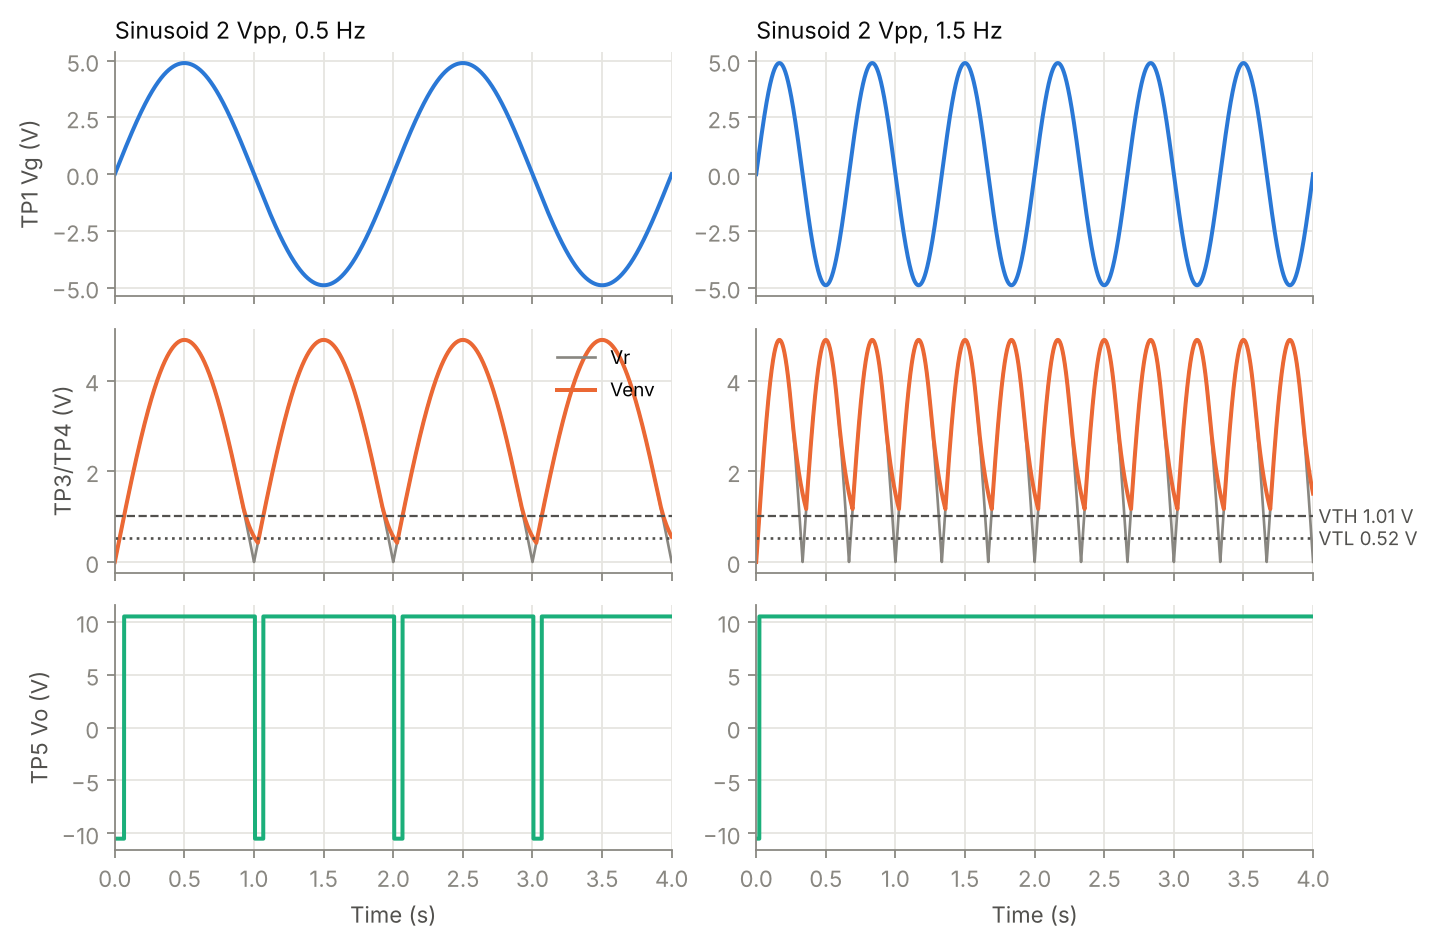
\includegraphics[width=0.95\linewidth]{f6_sinusoide.png}
\caption{\SI{2}{V_{pp}} sine wave at \SI{0.5}{Hz} (two pulses per cycle) and at \SI{1.5}{Hz} (output stuck high).}\label{fig:sin}
\end{figure}

\begin{table}[H]
\centering
\caption{Results with a sine wave (minimum of $\Venv$ in parentheses).}\label{tab:sin}
\begin{tabular}{@{}cccc@{}}
\toprule
Frequency & \SI{0.5}{V_{pp}} & \SI{1}{V_{pp}} & \SI{2}{V_{pp}} \\
\midrule
\SI{0.5}{Hz} & 2 pulses/cycle (0.11 V) & 2 pulses/cycle (0.21 V) & 2 pulses/cycle (0.42 V) \\
\SI{1.0}{Hz} & 2 pulses/cycle (0.20 V) & 2 pulses/cycle (0.41 V) & Stuck high (0.82 V) \\
\SI{1.5}{Hz} & 2 pulses/cycle (0.29 V) & Stuck high (0.58 V) & Stuck high (1.17 V) \\
\bottomrule
\end{tabular}
\end{table}

\begin{figure}[H]
\centering
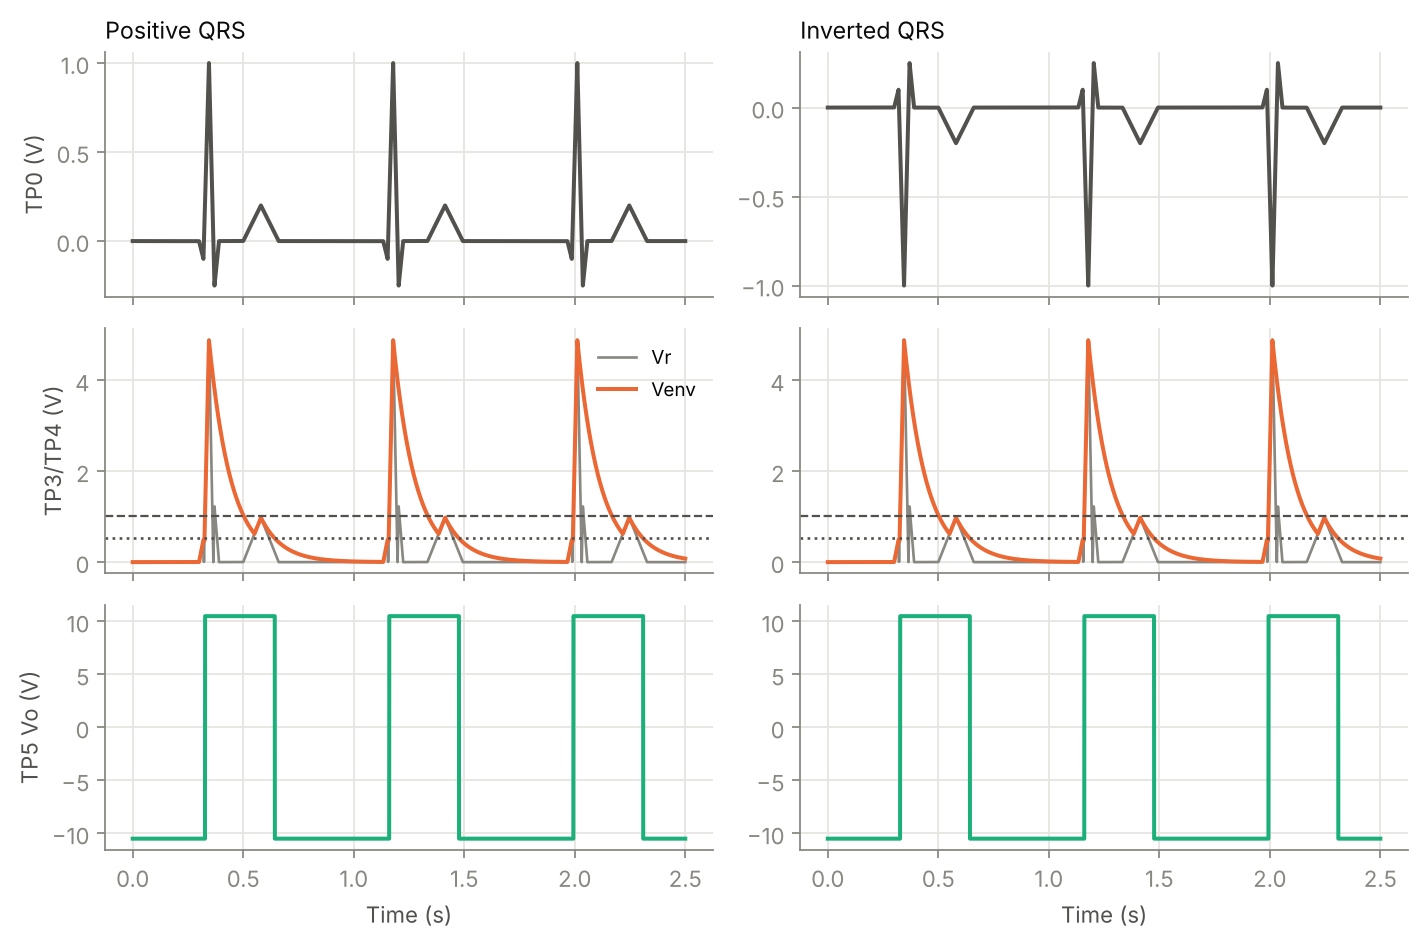
\includegraphics[width=0.95\linewidth]{f7_qrs_pwlin.png}
\caption{Synthetic heartbeat with positive and inverted QRS: a single pulse per beat in both cases.}\label{fig:qrs}
\end{figure}

With a synthetic heartbeat (a \SI{1}{V} QRS with negative Q and S waves and a \SI{0.2}{V} T wave) the circuit gives one pulse per beat for both polarities. After the gain, the T wave reaches \SI{0.98}{V}, just below $\VTH$, and it arrives while $\Venv$ is still above $\VTL$, so it only lengthens the pulse.

\subsection{Proteus simulation}

\paragraph{Op-amp model.} The LM741 model was used in Proteus (one amplifier per IC, pin 7 to $+\SI{12}{V}$ and pin 4 to $-\SI{12}{V}$). At the frequencies of this circuit its relevant parameters (slew rate of \SI{0.5}{V/\micro s}, $\Vsat\approx\pm\SI{10}{V}$, bias current of about \SI{80}{nA}) are equivalent to those of the LM324 and TL074 used in the build.

\paragraph{Simulated schematic.} Figure~\ref{fig:proteusesq} shows the circuit built in Proteus. The IC designators were assigned by the program and do not match those in this report; the correspondence is given in Table~\ref{tab:equiv}. Channel D of the oscilloscope is connected after D5 (LED node), which is why the low level of the output reads \SI{0}{V} instead of $-\Vsat$ in the screenshots.

\begin{table}[H]
\centering
\caption{Correspondence between the report numbering and the Proteus numbering.}\label{tab:equiv}
\begin{tabular}{@{}lll@{}}
\toprule
Function & Report & Proteus \\
\midrule
Amplifier & U1 & U1 \\
Half-wave & U2 & U5 \\
Summer & U3 & U4 \\
Detector & U4 & U9 \\
Buffer & U5 & U2 \\
Schmitt & U6 & U7 \\
LED & LED1 & D6 (LED-AQUA) \\
\bottomrule
\end{tabular}
\end{table}

\paragraph{Test sources.}
\begin{itemize}
  \item \textbf{PULSE:} low level \SI{0}{V}; high level 0.5, 1 or \SI{2}{V} ($-\SI{1}{V}$ for negative polarity); \SI{10}{\micro s} edges; width of \SI{9}{\percent} of the period or a fixed \SI{75}{ms}. The result screenshots were taken at \SI{0.5}{Hz} with \SI{9}{\percent} (\SI{180}{ms}).
  \item \textbf{SINE:} offset 0, peak-to-peak amplitude of 0.5 to \SI{2}{V}, frequency \SI{0.5}{Hz} (and 1 or \SI{1.5}{Hz} to show the limit set by $\tau$).
  \item \textbf{FILE:} text file with 12 synthetic heartbeats (time and voltage), with the \emph{Repeat Waveform} option enabled.
\end{itemize}

\paragraph{Instruments.} Virtual oscilloscope with A at the input or TP1, B at TP3, C at TP4 and D at TP5, all DC-coupled; time base of \SI{200}{ms/div} (\SI{500}{ms/div} for the sine wave) and rising-edge trigger on channel A.

\paragraph{Frequency scaling.} If the real-time simulation is slow, all frequencies are multiplied by $k$ and C1 is divided by $k$ (it is the only component that sets timing). With $k=10$: a \SI{12}{Hz} pulse, C1 $=\SI{100}{nF}$; the measured times are multiplied by 10.

\begin{landscape}
\begin{center}
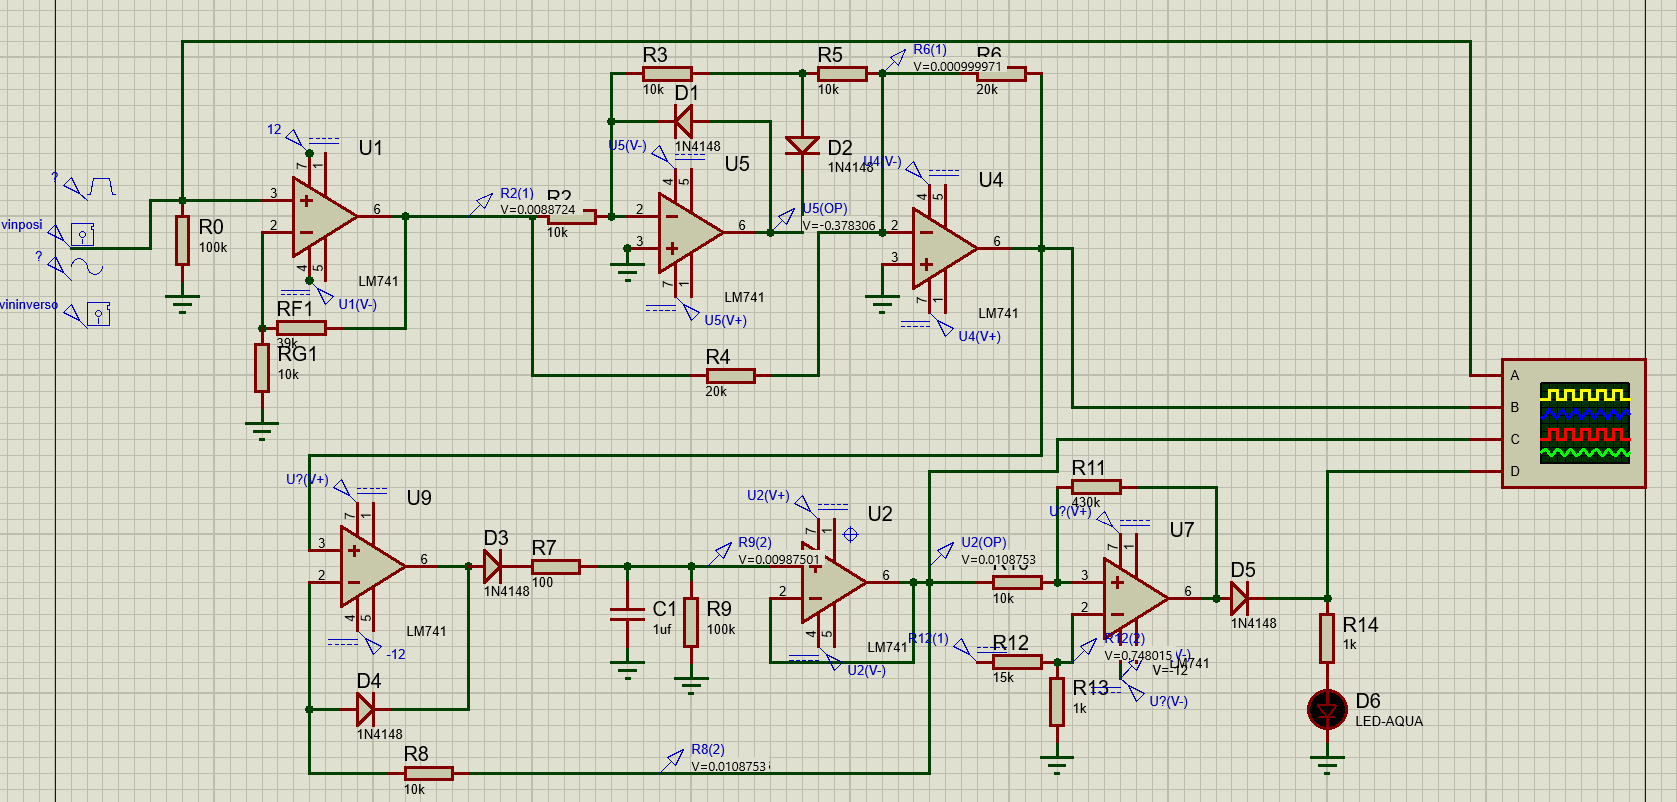
\includegraphics[width=\linewidth]{proteus_esquema.png}
\captionof{figure}{Circuit simulated in Proteus with LM741 op-amps and a virtual oscilloscope (A: input, B: $\Vr$, C: $\Venv$, D: output after D5).}\label{fig:proteusesq}
\end{center}
\end{landscape}

% ---------------------------- 7. PROCEDURE ---------------------------
\section{Experimental Procedure}

\subsection{Assembly}
\begin{enumerate}
  \item Power the ICs from $\pm\SI{12}{V}$ and place a \SI{100}{nF} capacitor between each supply pin and ground.
  \item Build and verify one stage at a time: check TP1 before connecting the rectifier, and so on.
  \item Use a common ground for the power supply, generator and oscilloscope.
  \item Check the orientation of D1 to D4: a reversed diode in the rectifier gives a half-wave output or leaves the output stuck at a rail.
  \item The circuit is intended only for tests with a generator; it is not connected to electrodes on a person, since that requires isolation and safety standards (IEC 60601).
\end{enumerate}

\subsection{Agilent 33120A generator setup}
The initial plan was to use the GW Instek AFG-2025 generator, which only offers pulses and sine waves. In the laboratory it was replaced by the Agilent 33120A because it has a built-in cardiac waveform (CARDIAC) with P, QRS and T waves, much closer to the real signal than the rectangular pulse. The sine wave was generated with the same instrument. The setup was:
\begin{enumerate}
  \item \textbf{Waveform:} \texttt{Shift} + \texttt{Arb} (\textit{Arb List}), select \texttt{CARDIAC} with the arrow keys, \texttt{Enter}, and then \texttt{Arb} to activate it.
  \item \textbf{Frequency:} \texttt{Freq}, \texttt{Enter Number}, \texttt{1.2} and the Hz unit arrow key. \SI{1.2}{Hz} corresponds to 72 bpm.
  \item \textbf{Amplitude:} \texttt{Ampl}, with 1, 2 and \SI{4}{V_{pp}} in the different tests.
  \item \textbf{High-impedance output termination} (\texttt{OUT TERM} $=$ \texttt{HIGH Z} in the system menu): by default the instrument assumes a \SI{50}{\ohm} load and, since the circuit input is \SI{100}{k\ohm}, it would deliver twice the displayed value.
  \item \textbf{Offset:} adjusted while watching the input on the oscilloscope with DC coupling, until the baseline between beats sat at \SI{0}{V}. If the baseline is negative, the rectifier turns it into a constant positive level and the envelope never falls below $\VTL$.
\end{enumerate}

\subsection{Measurement points}

\begin{table}[H]
\centering
\caption{Test points.}\label{tab:tp}
\begin{tabularx}{\linewidth}{@{}llX@{}}
\toprule
TP & Node & What to measure \\
\midrule
TP0 & Input & Actual $V_{pp}$, frequency and pulse width \\
TP1 & U1 output ($\Vg$) & Amplitude and actual gain \\
TP2 & Half-wave ($V_{hw}$) & Only the positive half-cycle of $\Vg$, inverted \\
TP3 & U3 output ($\Vr$) & $|\Vg|$, with no step at the zero crossing \\
TP4 & U5 output ($\Venv$) & Peak and $\tau$ (time to \SI{37}{\percent} of the peak) \\
TP5 & U6 output & $\pm\Vsat$ levels, pulse width and frequency \\
\bottomrule
\end{tabularx}
\end{table}

With a two-channel oscilloscope, measurements are taken in consecutive pairs (TP0--TP1, TP1--TP3, TP3--TP4, TP4--TP5) triggering on channel 1. The thresholds are measured in XY mode ($X=$ TP4, $Y=$ TP5) with a slow ramp at the Schmitt input. The offset is measured at TP4 with the input at \SI{0}{V}.

% ---------------------------- 8. RESULTS -----------------------------
\section{Results}

\subsection{Proteus simulation}

\paragraph{\SI{1}{V} pulse at \SI{0.5}{Hz}.} With a \SI{9}{\percent} duty cycle the pulse lasts $w=0.09\times\SI{2}{s}=\SI{180}{ms}$. The expected output width is
\begin{equation}
w+\tau\ln\frac{V_p}{\VTL}=\SI{180}{ms}+\SI{100}{ms}\cdot\ln\frac{4.95}{0.523}=\SI{180}{ms}+\SI{225}{ms}=\SI{405}{ms}
\end{equation}
In the screenshot (Figure~\ref{fig:proteuspulso}) the output stays high for about \SI{400}{ms}, $\Vr$ reaches \SI{4.90}{V} and $\Venv$ \SI{4.95}{V}; the envelope stays flat during the pulse and then decays exponentially.

\begin{figure}[H]
\centering
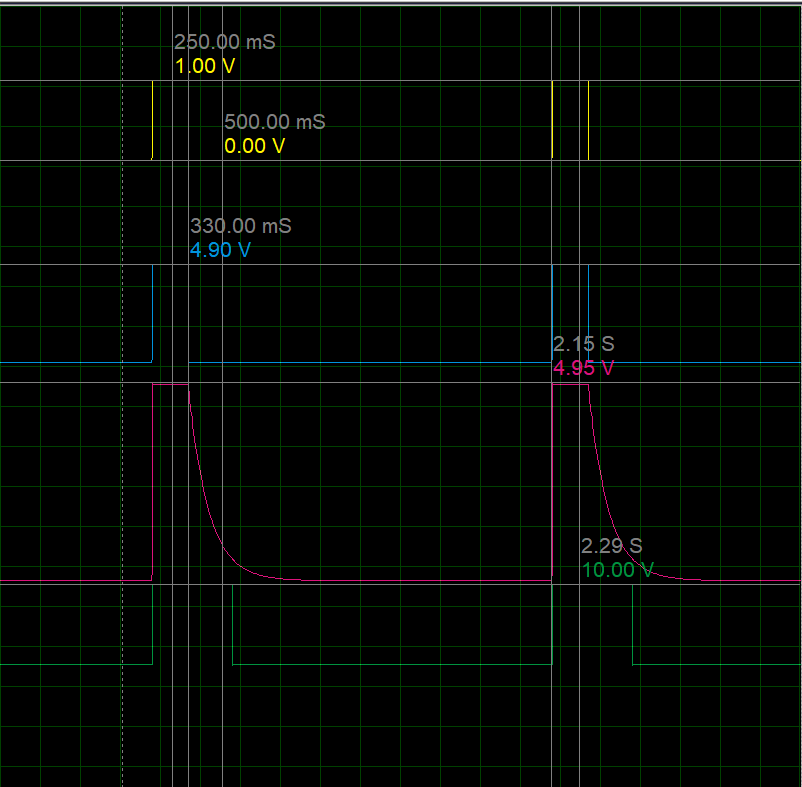
\includegraphics[width=0.78\linewidth]{proteus_pulso.png}
\caption{Proteus, \SI{1}{V} pulse at \SI{0.5}{Hz}. Yellow: input; blue: $\Vr$ (TP3); pink: $\Venv$ (TP4); green: output after D5.}\label{fig:proteuspulso}
\end{figure}

\paragraph{\SI{2}{V_{pp}} sine wave at \SI{0.5}{Hz}.} $\Vr$ shows the two positive humps per cycle with a \SI{4.90}{V} peak, which confirms full-wave rectification. The output is high almost all the time and drops briefly near each zero crossing, when $\Venv$ falls below $\VTL$: there are two rising edges per cycle, one per half-cycle (Figure~\ref{fig:proteusseno}).

\begin{figure}[H]
\centering
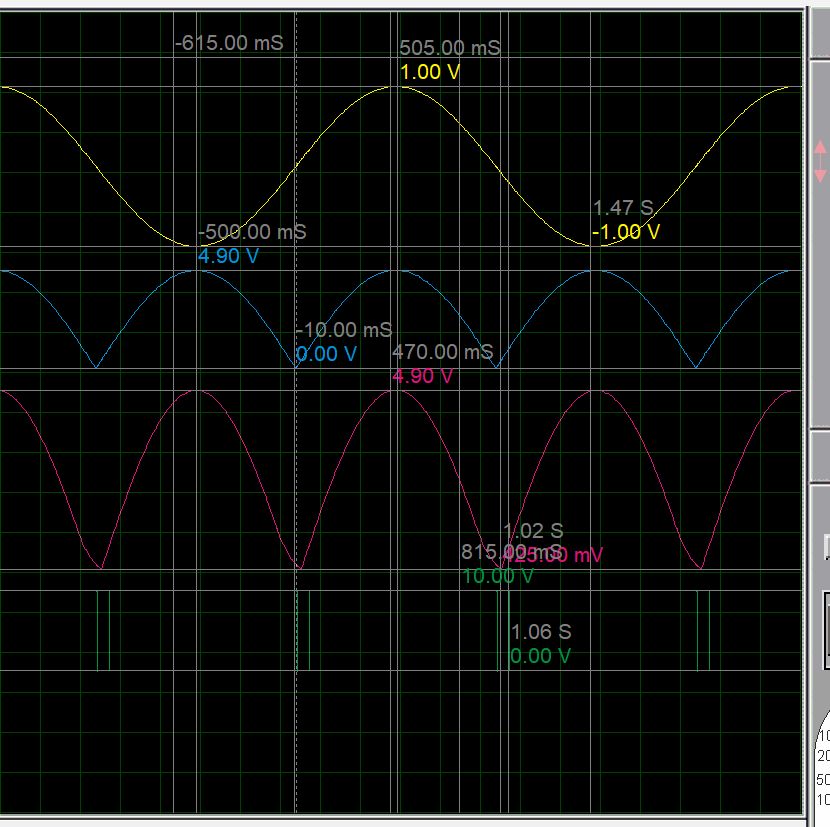
\includegraphics[width=0.78\linewidth]{proteus_seno.png}
\caption{Proteus, \SI{2}{V_{pp}} sine wave at \SI{0.5}{Hz}: two output pulses per cycle.}\label{fig:proteusseno}
\end{figure}

\paragraph{Synthetic heartbeat (FILE generator).} With the 12-beat file (\SI{1}{V} QRS, negative Q and S waves and a \SI{0.2}{V} T wave), $\Vr$ shows the rectified lobes and the T wave, but $\Venv$ merges them into a single hump per beat. The output gives one pulse of about \SI{325}{ms} per beat, and the T wave causes no false triggers (Figure~\ref{fig:proteusecg}).

\begin{figure}[H]
\centering
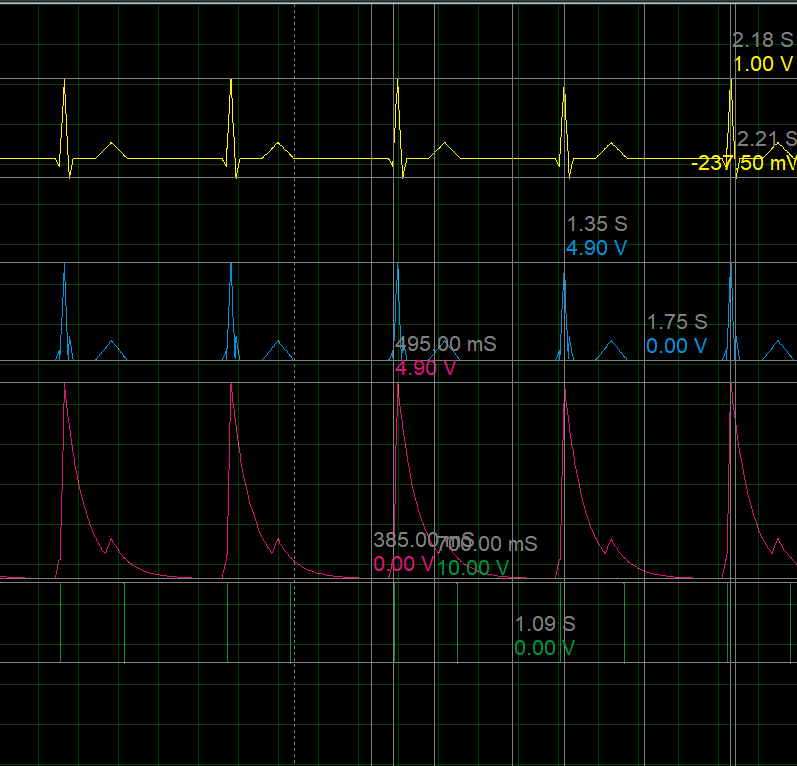
\includegraphics[width=0.78\linewidth]{proteus_ecg.png}
\caption{Proteus, synthetic heartbeat at 72 bpm: one output pulse per beat.}\label{fig:proteusecg}
\end{figure}

\begin{table}[H]
\centering
\caption{Comparison of theoretical values, Proteus simulation and laboratory measurements.}\label{tab:comparacion}
\small
\begin{tabular}{@{}lcccc@{}}
\toprule
Quantity & Theoretical & Proteus & Error (\%) & Measured \\
\midrule
\multicolumn{5}{@{}l}{\textit{\SI{1}{V} pulse, \SI{0.5}{Hz}, \SI{180}{ms} wide}} \\
Gain $\Vr/V_{in}$ & 4.90 & 4.90 & 0.0 & \\
Peak of $\Vr$ (TP3) & \SI{4.90}{V} & \SI{4.90}{V} & 0.0 & \\
Peak of $\Venv$ (TP4) & \SI{4.90}{V} & \SI{4.95}{V} & 1.0 & \\
Output pulse width & \SI{405}{ms} & $\approx\SI{400}{ms}$ & 1.2 & \\
Output period & \SI{2}{s} (30 bpm) & \SI{2}{s} & 0.0 & \\
\midrule
\multicolumn{5}{@{}l}{\textit{\SI{2}{V_{pp}} sine wave, \SI{0.5}{Hz}}} \\
Peak of $\Vr$ & \SI{4.90}{V} & \SI{4.90}{V} & 0.0 & \\
Pulses per cycle & 2 & 2 & --- & \\
\midrule
\multicolumn{5}{@{}l}{\textit{Synthetic heartbeat, 72 bpm}} \\
Pulses per beat & 1 & 1 & --- & \\
Output pulse width & $\approx\SI{320}{ms}$ & $\approx\SI{325}{ms}$ & 1.6 & \\
\midrule
\multicolumn{5}{@{}l}{\textit{Additional laboratory measurements}} \\
Discharge $\tau$ & \SI{100}{ms} & & & \\
$\VTH$ & \SI{1.01}{V} & & & \\
$\VTL$ & \SI{0.52}{V} & & & \\
Offset at TP4 (input at \SI{0}{V}) & $<\SI{50}{mV}$ & & & \\
\bottomrule
\end{tabular}
\end{table}

\subsection{Laboratory build}

The circuit was built on a breadboard with two LM324N chips powered from $\pm\SI{12}{V}$ by a dual supply in series mode, with a common ground for the supply, generator and oscilloscope (Figure~\ref{fig:montaje}).

\begin{figure}[H]
\centering
\begin{subfigure}[b]{0.49\linewidth}\centering
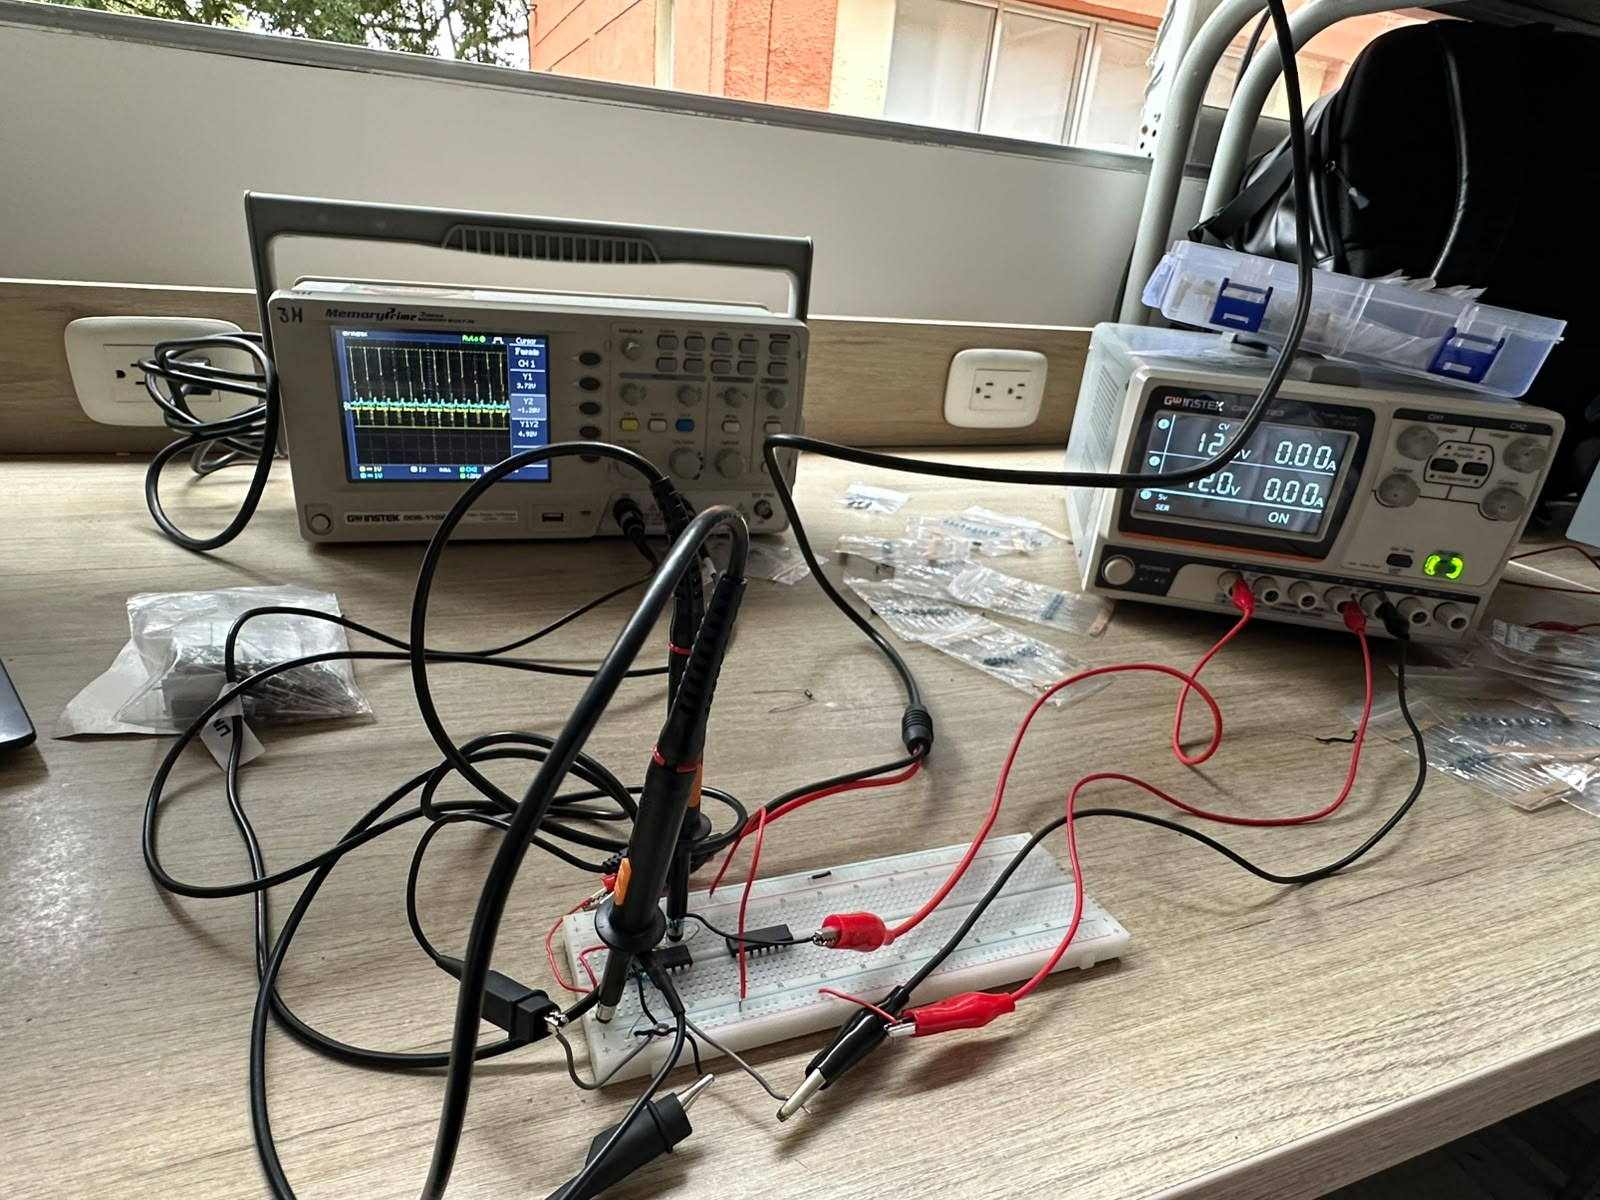
\includegraphics[width=\linewidth]{lab_banco.jpg}
\caption{Test bench: oscilloscope, dual supply and breadboard.}
\end{subfigure}\hfill
\begin{subfigure}[b]{0.49\linewidth}\centering
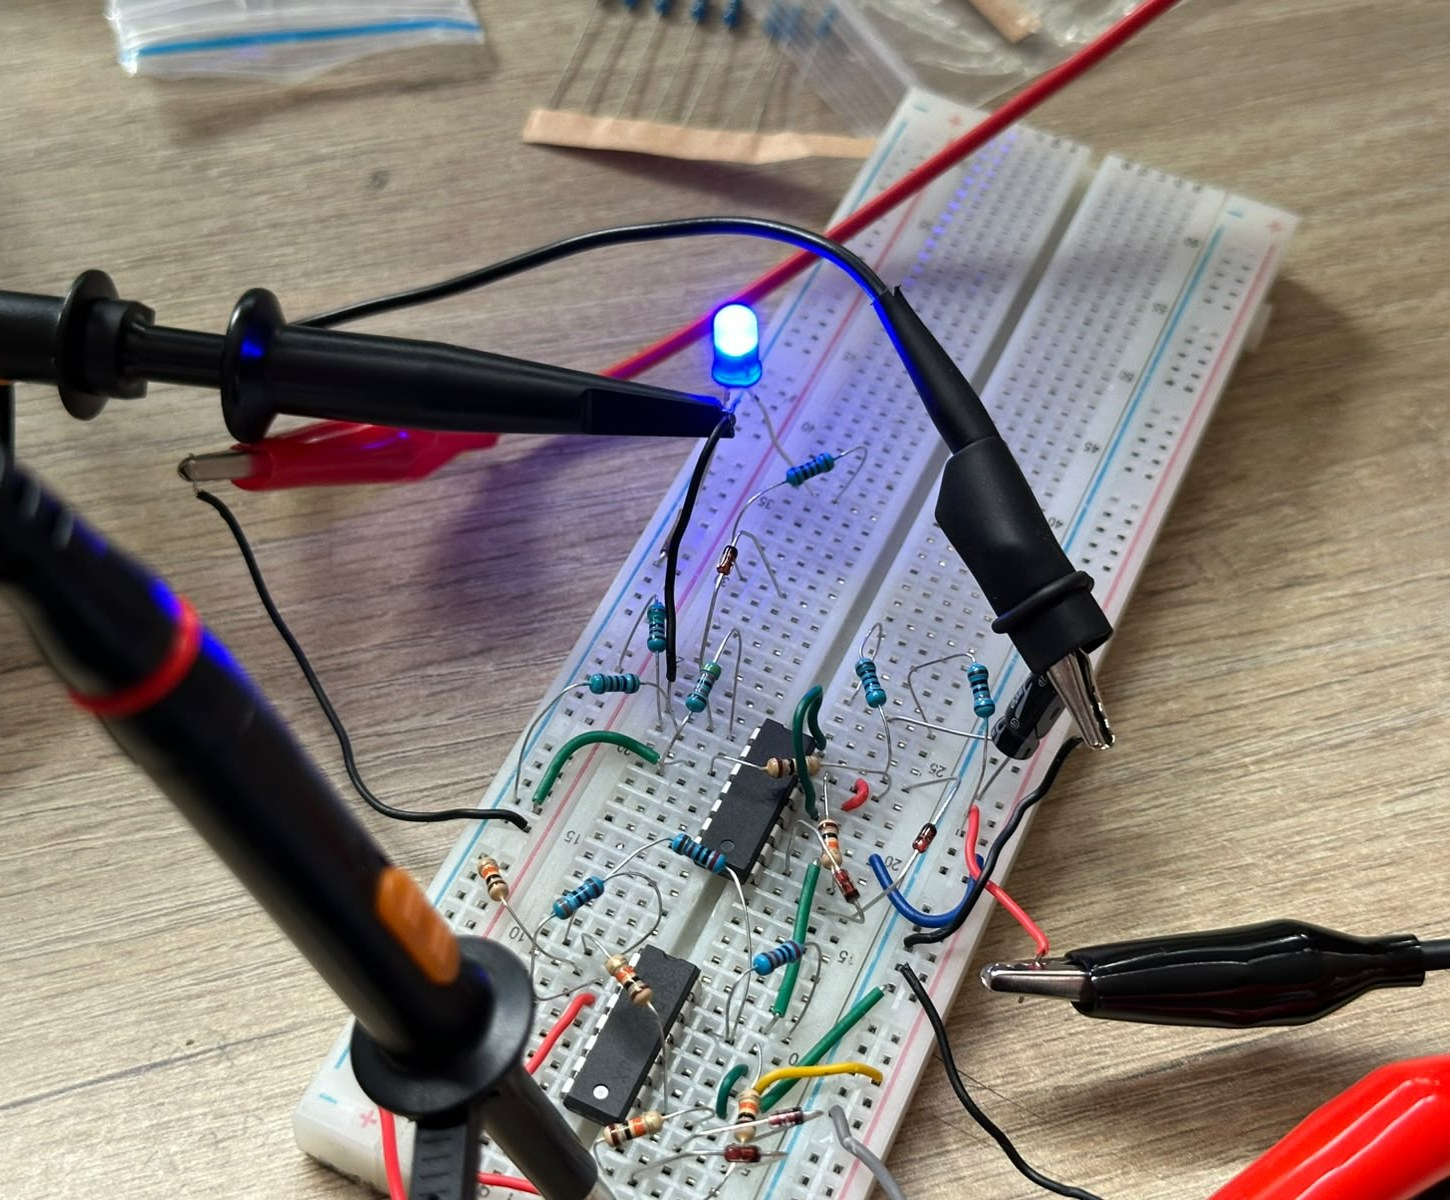
\includegraphics[width=\linewidth]{lab_montaje_led.jpg}
\caption{Build with two LM324N chips; LED lit during a beat.}
\end{subfigure}
\caption{The detector built in the laboratory.}\label{fig:montaje}
\end{figure}

\subsubsection{Input signal}
Figure~\ref{fig:labentrada} shows the \SI{1}{V_{pp}} CARDIAC waveform measured at the input with DC coupling. The P wave, the QRS and the T wave can be distinguished, with the baseline at \SI{0}{V}. The R peak reaches \SI{0.78}{V} and the S wave $-\SI{0.22}{V}$, with \SI{1.00}{V} between cursors, equal to the value programmed on the generator.

\begin{figure}[H]
\centering
\begin{subfigure}[b]{0.55\linewidth}\centering
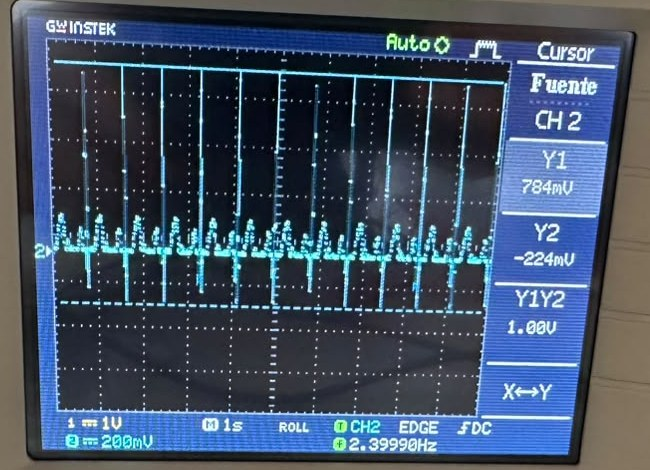
\includegraphics[width=\linewidth]{lab_entrada_cardiac.jpg}
\caption{Input (\SI{200}{mV/div}, \SI{1}{s/div}).}
\end{subfigure}\hfill
\begin{subfigure}[b]{0.43\linewidth}\centering
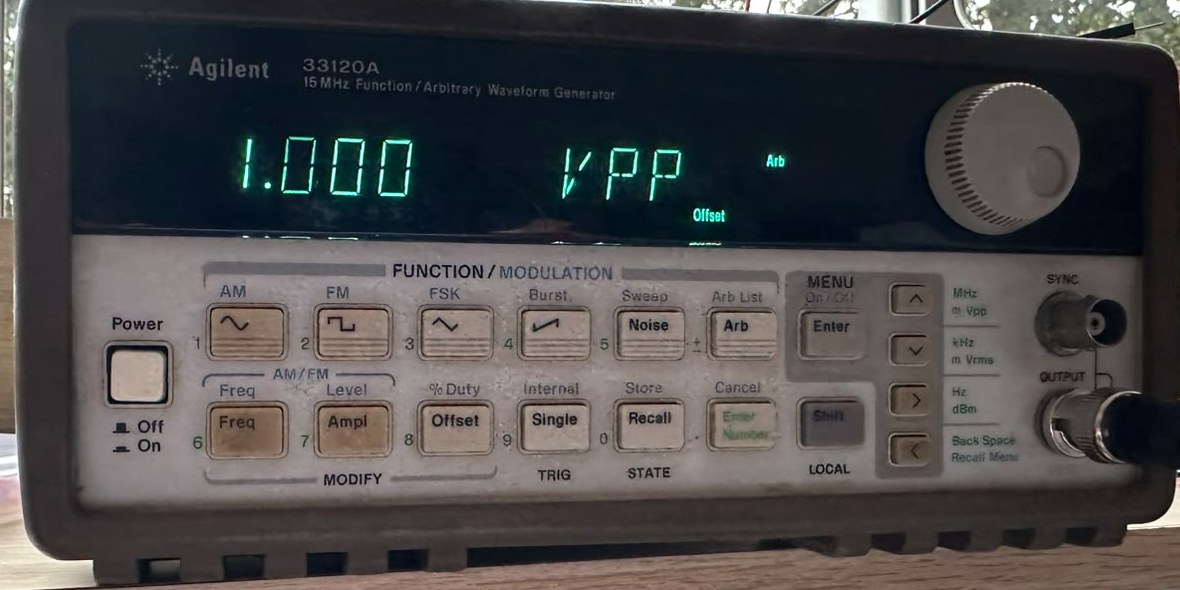
\includegraphics[width=\linewidth]{lab_gen_1vpp.jpg}
\caption{Generator set to \SI{1.000}{V_{pp}}, \textit{Arb} waveform.}
\end{subfigure}
\caption{Cardiac test signal from the Agilent 33120A.}\label{fig:labentrada}
\end{figure}

\subsubsection{Stage-by-stage response to the cardiac signal (\SI{1}{V_{pp}}, \SI{1.2}{Hz})}

\begin{figure}[H]
\centering
\begin{subfigure}[b]{0.49\linewidth}\centering
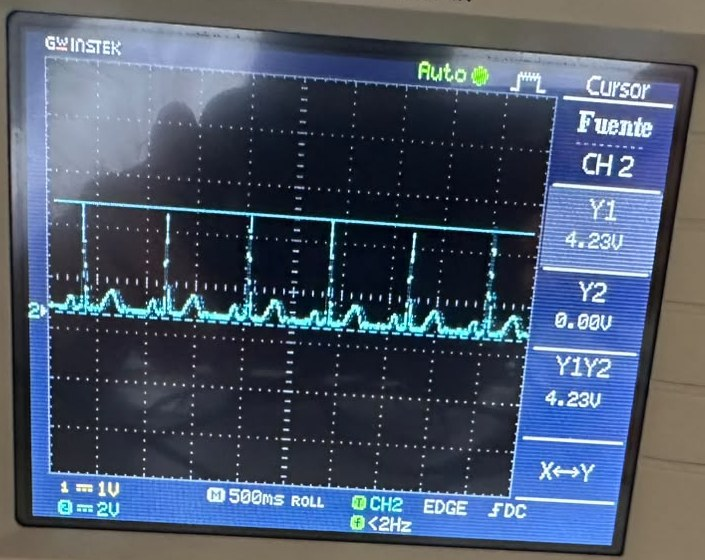
\includegraphics[width=\linewidth]{lab_vr_ecg.jpg}
\caption{TP3, $\Vr$ (\SI{2}{V/div}, \SI{500}{ms/div}).}
\end{subfigure}\hfill
\begin{subfigure}[b]{0.49\linewidth}\centering
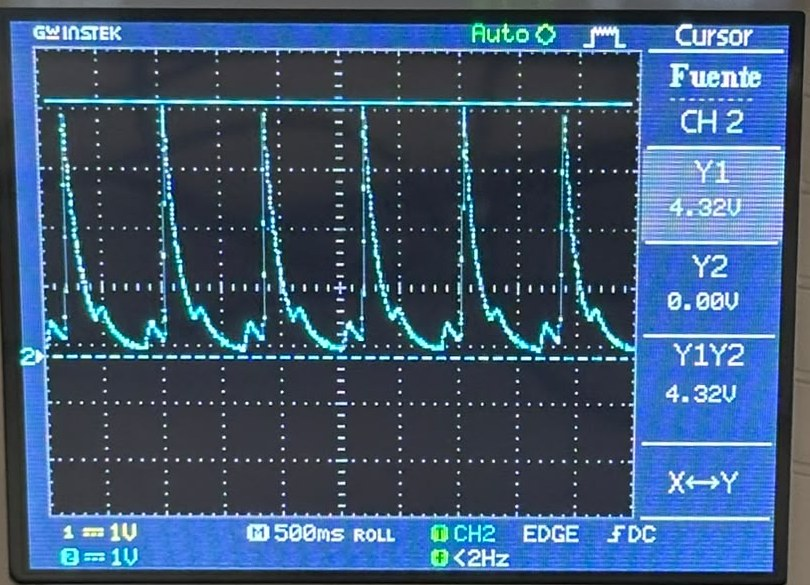
\includegraphics[width=\linewidth]{lab_venv_ecg.jpg}
\caption{TP4, $\Venv$ (\SI{1}{V/div}, \SI{500}{ms/div}).}
\end{subfigure}
\caption{Rectifier and peak detector outputs with the cardiac signal.}\label{fig:labetapas}
\end{figure}

\begin{itemize}
  \item \textbf{Rectifier (TP3):} the whole signal becomes positive and the baseline stays at \SI{0}{V}, with no step at the zero crossing. The rectified R peak reaches \SI{4.23}{V}. With the design gain and the input peak read in Figure~\ref{fig:labentrada}, $4.9\times0.78=\SI{3.84}{V}$ was expected. The difference, about \SI{10}{\percent}, is attributed mainly to the fact that at \SI{1}{s/div} in \textit{roll} mode the oscilloscope takes few samples per division and clips the R peak, which lasts a few tens of milliseconds. The tolerance of Rf1 and Rg1 (\SI{5}{\percent}) also contributes.
  \item \textbf{Peak detector (TP4):} the envelope rises with the QRS up to \SI{4.32}{V} and discharges exponentially. The \SI{0.09}{V} difference with respect to $\Vr$ is the accumulated offset of U4 and U5, of the same order as observed in Proteus. The rectified T wave appears as a small hump during the discharge.
\end{itemize}

\subsubsection{Comparator output}

\begin{figure}[H]
\centering
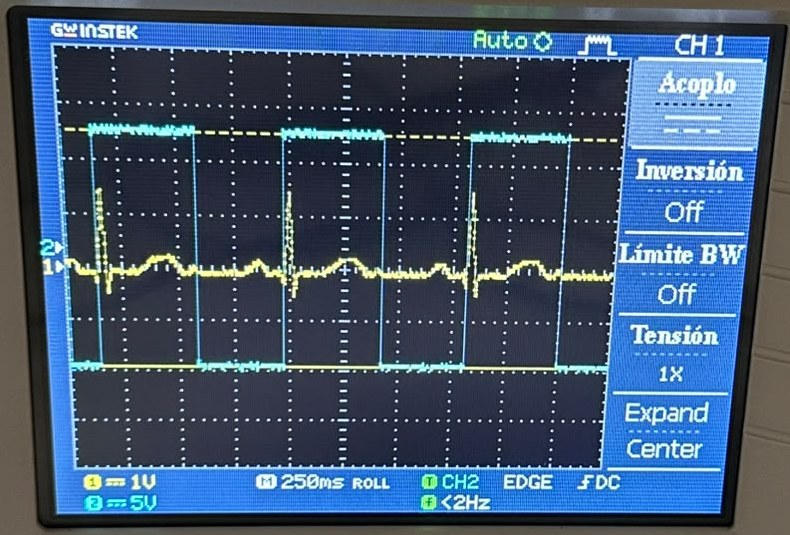
\includegraphics[width=0.75\linewidth]{lab_entrada_salida.jpg}
\caption[Cardiac input and Schmitt output at TP5]{Cardiac input (CH1, yellow, \SI{1}{V/div}) and Schmitt output at TP5 (CH2, blue, \SI{5}{V/div}), at \SI{250}{ms/div}: one rectangular pulse for each QRS.}\label{fig:labsalida}
\end{figure}

Figure~\ref{fig:labsalida} is the main result of the build: each QRS at the input produces a single rising edge at the output, and the T wave does not generate extra triggers. The output switches between the saturation levels of the LM324N. As measured with the oscilloscope (Figure~\ref{fig:labmedidas}a), the high level is \SI{11.1}{V} and the output frequency is \SI{1.199}{Hz}, equal to that of the input. With this high level, the actual thresholds are $\VTH=0.767+11.1\,(0.02326)=\SI{1.03}{V}$ and $\VTL=\SI{0.51}{V}$, within \SI{20}{mV} of the design values. Measured after D5, across the LED, the output goes from \SI{0}{V} to \SI{9.9}{V} (Figure~\ref{fig:labled}): D5 blocks the negative level, as designed.

\begin{figure}[H]
\centering
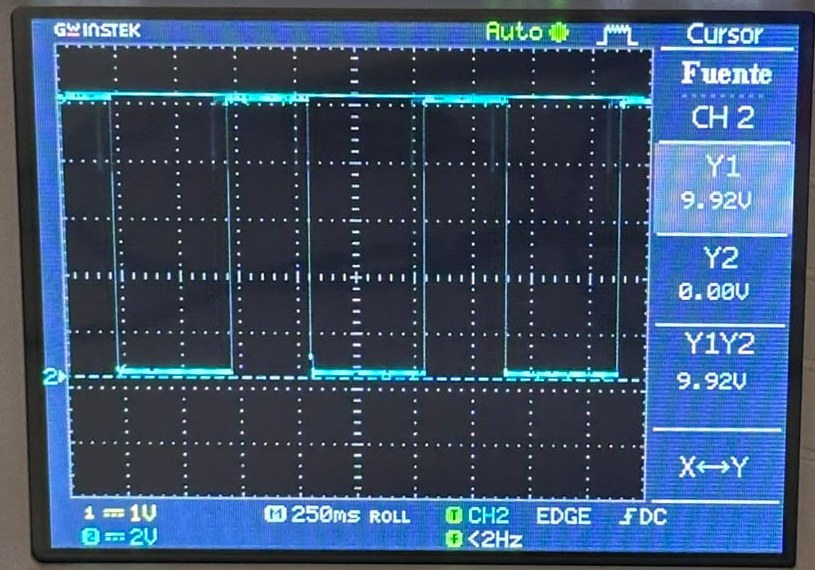
\includegraphics[width=0.6\linewidth]{lab_salida_led.jpg}
\caption{Output measured after D5, across the LED (\SI{2}{V/div}, \SI{250}{ms/div}): from \SI{0}{V} to \SI{9.92}{V}.}\label{fig:labled}
\end{figure}

\subsubsection{Test with \SI{4}{V_{pp}} at \SI{1.2}{Hz}}
To check the robustness of the design, the amplitude was increased to 2 and then to \SI{4}{V_{pp}}, twice the specified maximum. At \SI{1.2}{Hz} the circuit kept delivering one pulse per beat, with \SI{1.202}{Hz} measured at the output (Figure~\ref{fig:labmedidas}b).

\begin{figure}[H]
\centering
\begin{subfigure}[b]{0.49\linewidth}\centering
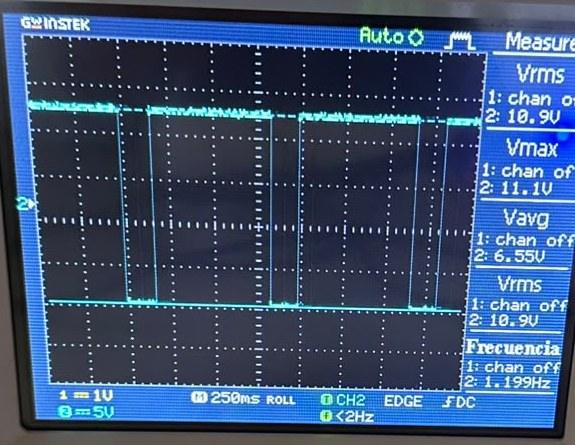
\includegraphics[width=\linewidth]{lab_medida_a.jpg}
\caption{\SI{1}{V_{pp}}: $V_{max}=\SI{11.1}{V}$, $V_{avg}=\SI{6.55}{V}$, \SI{1.199}{Hz}.}
\end{subfigure}\hfill
\begin{subfigure}[b]{0.49\linewidth}\centering
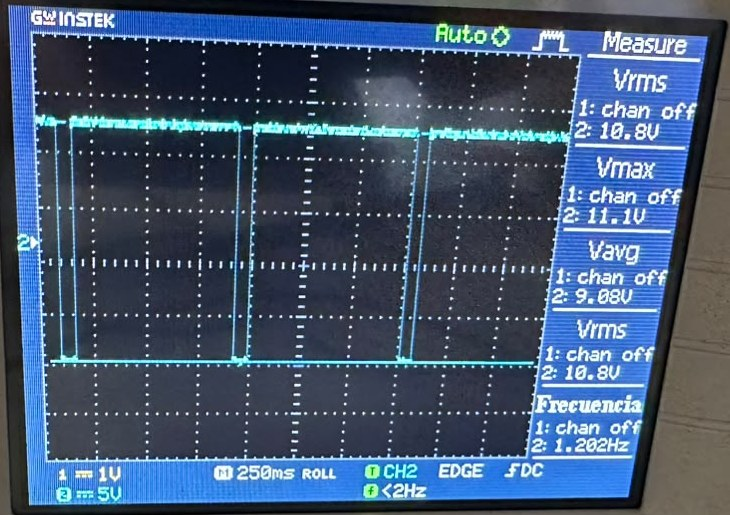
\includegraphics[width=\linewidth]{lab_medida_b.jpg}
\caption{\SI{4}{V_{pp}}: $V_{max}=\SI{11.1}{V}$, $V_{avg}=\SI{9.08}{V}$, \SI{1.202}{Hz}.}
\end{subfigure}
\caption{Automatic measurements of the Schmitt output (TP5, \SI{5}{V/div}, \SI{250}{ms/div}).}\label{fig:labmedidas}
\end{figure}

\begin{figure}[H]
\centering
\begin{subfigure}[b]{0.52\linewidth}\centering
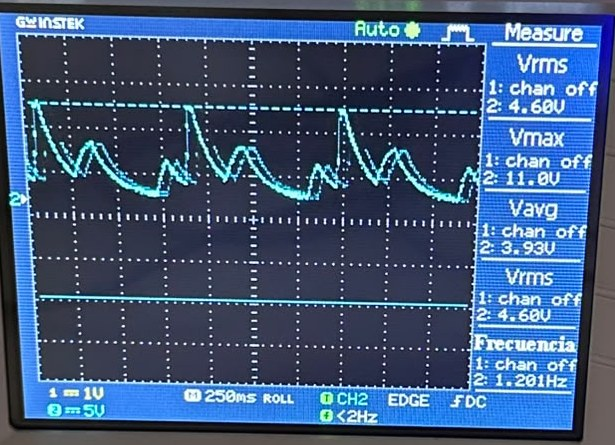
\includegraphics[width=\linewidth]{lab_venv_4vpp.jpg}
\caption{$\Venv$ with \SI{4}{V_{pp}}: saturates at \SI{11.0}{V}.}
\end{subfigure}\hfill
\begin{subfigure}[b]{0.46\linewidth}\centering
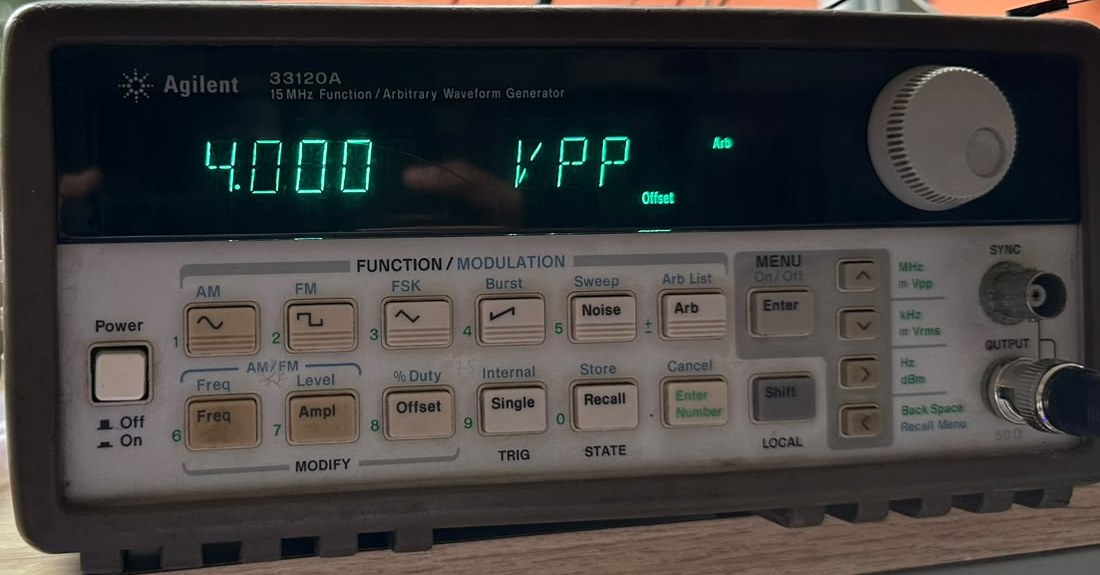
\includegraphics[width=\linewidth]{lab_gen_4vpp.jpg}
\caption{Generator set to \SI{4.000}{V_{pp}}.}
\end{subfigure}
\caption{Out-of-specification test: \SI{4}{V_{pp}} input at \SI{1.2}{Hz}.}\label{fig:lab4vpp}
\end{figure}

Since the output alternates between $+V_H\approx\SI{11.1}{V}$ and $-V_L\approx\SI{10.5}{V}$, the duty cycle $d$ is obtained from the measured average value, $V_{avg}=d\,V_H-(1-d)\,V_L$:
\begin{equation}
d=\frac{V_{avg}+V_L}{V_H+V_L}
\end{equation}

\begin{table}[H]
\centering
\caption{Comparator output with the cardiac signal at \SI{1.2}{Hz} ($T\approx\SI{833}{ms}$).}\label{tab:labsalida}
\small
\begin{tabular}{@{}lcccccc@{}}
\toprule
Input & $\Venv$ peak & $f_{out}$ & $V_{avg}$ & $d$ & Time high & Time low \\
\midrule
\SI{1}{V_{pp}} & \SI{4.32}{V} & \SI{1.199}{Hz} & \SI{6.55}{V} & \SI{79}{\percent} & \SI{658}{ms} & \SI{176}{ms} \\
\SI{4}{V_{pp}} & \SI{11.0}{V} (saturated) & \SI{1.202}{Hz} & \SI{9.08}{V} & \SI{91}{\percent} & \SI{754}{ms} & \SI{78}{ms} \\
\bottomrule
\end{tabular}
\end{table}

Two effects explain why the circuit tolerates \SI{4}{V_{pp}} at 72 bpm:
\begin{itemize}
  \item \textbf{Saturation limits the envelope.} With \SI{4}{V_{pp}}, U1 saturates and $\Venv$ does not exceed about \SI{11}{V}. The discharge time is bounded to $\tau\ln(11/0.52)\approx\SI{305}{ms}$ even if the input keeps growing, and the comparator manages to release within the \SI{833}{ms} period.
  \item \textbf{The T wave lengthens the pulse.} With the cardiac waveform the output pulse lasts considerably longer than with the \SI{75}{ms} rectangular pulse (\SI{658}{ms} versus about \SI{300}{ms}), because the rectified T wave recharges C1 and keeps $\Venv$ above $\VTL$. With \SI{4}{V_{pp}} the amplified T wave is larger and the time low shrinks to \SI{78}{ms}: the circuit still works, but close to its limit. At higher rates or amplitudes the beats would start to merge.
\end{itemize}
When U1 saturates, the amplitude information is lost, but detection does not depend on it: it is enough for $\Venv$ to exceed $\VTH$ and fall back below $\VTL$ in every period.

\subsubsection{Sine-wave test}

\begin{figure}[H]
\centering
\begin{subfigure}[b]{0.49\linewidth}\centering
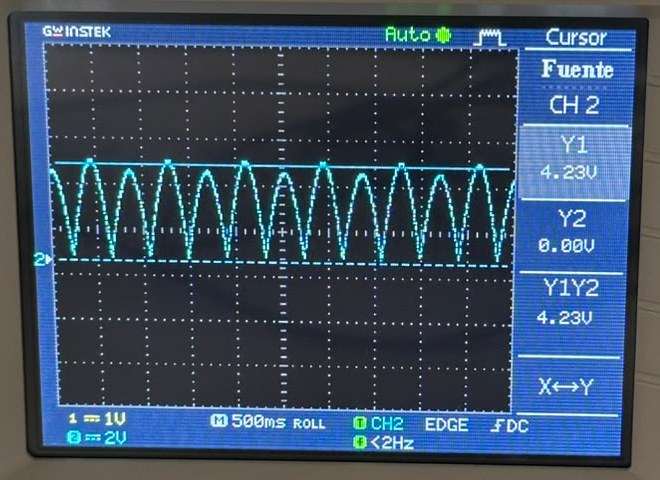
\includegraphics[width=\linewidth]{lab_vr_seno.jpg}
\caption{TP3, $\Vr$: full wave, \SI{4.23}{V} peak.}
\end{subfigure}\hfill
\begin{subfigure}[b]{0.49\linewidth}\centering
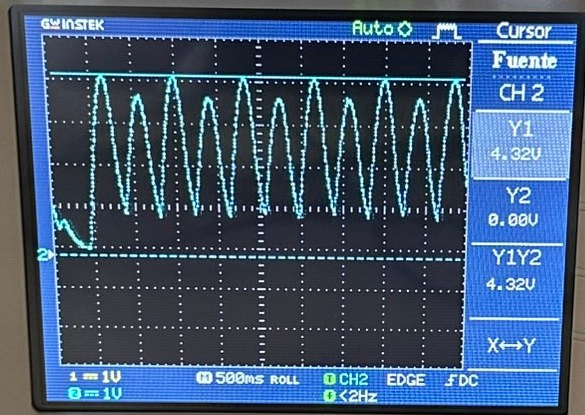
\includegraphics[width=\linewidth]{lab_venv_seno.jpg}
\caption{TP4, $\Venv$: oscillates between $\approx\SI{1.6}{V}$ and \SI{4.32}{V}.}
\end{subfigure}
\caption{Response to the sine wave (\SI{500}{ms/div}).}\label{fig:labseno}
\end{figure}

The rectifier delivers a clean full-wave signal, with two positive half-cycles per cycle and valleys that reach exactly \SI{0}{V}. This confirms on the actual build that the precision rectifier has no noticeable dead zone. The envelope, on the other hand, never drops below $\approx\SI{1.6}{V}$: the sine wave rises again before C1 discharges down to $\VTL$, so the comparator stays high and does not deliver separate pulses. This is the behavior anticipated by the sine-wave simulation: this type of signal has a much lower frequency limit than the pulse, because it produces two events per cycle and almost never sits at zero.

\subsubsection{Summary: calculation, simulation and build}

\begin{table}[H]
\centering
\caption{Comparison of results.}\label{tab:labcomparison}
\small
\begin{tabularx}{\linewidth}{@{}>{\raggedright}p{3.3cm}>{\raggedright}p{2.7cm}>{\raggedright}p{2.4cm}X@{}}
\toprule
Quantity & Calculation / Proteus & Build & Comment \\
\midrule
Output high level & \SI{10.5}{V} (assumed) & \SI{11.1}{V} & LM324N at $\pm\SI{12}{V}$ with a light load \\
$\VTH$ / $\VTL$ & 1.01 / \SI{0.52}{V} & 1.03 / \SI{0.51}{V} & Recalculated with the measured high level \\
Offset $\Venv-\Vr$ & \SI{0.05}{V} (Proteus) & \SI{0.09}{V} & Offset of U4 and U5 \\
$\Vr$ valley with sine wave & \SI{0}{V} & \SI{0}{V} & No dead zone \\
Pulses per beat & 1 & 1 & No triggers from the T wave \\
Output frequency & \SI{1.2}{Hz} & \SI{1.199}{Hz} & Equal to the input \\
Maximum amplitude tested & \SI{2}{V_{pp}} (design) & \SI{4}{V_{pp}} & Works thanks to U1 saturation \\
\bottomrule
\end{tabularx}
\end{table}

% ---------------------------- 9. ANALYSIS ----------------------------
\section{Analysis and Discussion}

\subsection{Frequency limits}
The upper limit is set by the condition $w+t_{desc}<T$ (equation~\ref{eq:fcmax}): with the fixed \SI{75}{ms} pulse width it is 262, 201 and 163 bpm for 0.5, 1 and \SI{2}{V_{pp}}. It decreases with amplitude because a larger peak takes longer to discharge: doubling the peak adds $\tau\ln2\approx\SI{69}{ms}$. There is no real lower limit, because the circuit is DC-coupled; the pulse only needs to last at least $\approx\SI{0.5}{ms}$ to charge C1. The sine wave has a lower limit than the pulse because it produces two events per cycle and the signal is almost never at zero.

\subsection{Op-amp comparison}\label{sec:opamps}

\begin{table}[H]
\centering
\caption{Op-amps considered.}\label{tab:opamps}
\begin{tabularx}{\linewidth}{@{}lllX@{}}
\toprule
Parameter & TL074 & LM324 / LM741 & Effect on the circuit \\
\midrule
Bias current & $\approx\SI{30}{pA}$ & 45--\SI{80}{nA} & Error on C1 below \SI{0.2}{\percent} in both cases \\
Slew rate & \SI{13}{V/\micro s} & \SI{0.5}{V/\micro s} & \si{\micro s} transitions: negligible \\
Output at $\pm\SI{12}{V}$ & $\pm\SI{10.5}{V}$ & $\approx\pm10$ to \SI{11.5}{V} & Shifts the thresholds by a few mV \\
Offset on $\Venv$ & 15--\SI{20}{mV} & 20--\SI{45}{mV} typical & Well below $\VTL$ \\
\bottomrule
\end{tabularx}
\end{table}

\subsection{Limitations}
\begin{itemize}
  \item Fixed thresholds: below $\approx\SI{0.4}{V_{pp}}$ there is no detection, and above $\approx\SI{2.1}{V_{pp}}$ U1 saturates. A real monitor uses an adaptive threshold (a fraction of the previous peak).
  \item A fixed $\tau$ limits the maximum rate to $\approx163$ bpm at \SI{2}{V_{pp}} for the rectangular pulse. With a cardiac waveform the limit is lower, because the T wave prolongs the envelope: in the build, with \SI{4}{V_{pp}} at 72 bpm, the comparator was low for only \SI{78}{ms} between beats.
  \item No filtering: with a real signal, a tall T wave or \SI{60}{Hz} noise could trigger the comparator. A real monitor places an instrumentation amplifier and a 0.5 to \SI{40}{Hz} band-pass filter in front.
  \item With the 741, the worst-case bias current through R0 can bring the offset to $\approx\SI{0.27}{V}$; if this is a problem, R0 can be lowered to \SI{10}{k\ohm} without affecting the rest of the circuit.
\end{itemize}

% ---------------------------- 10. CONCLUSIONS ------------------------
\section{Conclusions}
\begin{itemize}
  \item A heartbeat detector that delivers one pulse for every QRS complex was designed using only nonlinear op-amp blocks. In Proteus the values matched the calculated ones with errors of 1.6\% or less: peaks of \SI{4.90}{V} at $\Vr$ and \SI{4.95}{V} at $\Venv$, and an output pulse of about \SI{400}{ms} versus the predicted \SI{405}{ms}.
  \item The build with two LM324N chips met the objective with a realistic cardiac signal (CARDIAC waveform of the Agilent 33120A): one rectangular pulse per beat at \SI{1.199}{Hz}, with no triggers from the T wave. The actual high level was \SI{11.1}{V} instead of \SI{10.5}{V}, which shifts the thresholds by less than \SI{20}{mV}. With \SI{4}{V_{pp}} at \SI{1.2}{Hz}, twice the design maximum, the circuit kept detecting every beat, because op-amp saturation limits the envelope to about \SI{11}{V} and bounds the discharge time. However, the time low dropped to \SI{78}{ms}: with large amplitudes and a pronounced T wave the design operates close to its limit.
  \item The full-wave precision rectifier solved the polarity problem: the sine wave gave two pulses per cycle in Proteus, the inverted synthetic heartbeat was detected just like the positive one and, in the build, the full-wave signal reached exactly \SI{0}{V} at every valley. Placing the diode inside the feedback loop reduces the dead zone from \SI{0.6}{V} to a few \si{\micro V}; a passive rectifier would have lost \SI{25}{\percent} of the smallest signal.
  \item The summer shows how a linear operation produces a nonlinear function: combining the full signal (weight 1) with the half-wave signal (weight 2) gives $|\Vg|$. The analysis also showed that the positive half-cycle depends on a subtraction ($2-1$), so the resistors must be \SI{1}{\percent}.
  \item The discharge time constant $\tau=R_9C_1$ is the critical parameter. It was not chosen arbitrarily: the 90 to \SI{110}{ms} window comes from two opposing conditions, merging the QRS lobes and releasing the comparator before the next beat. The formula $HR_{max}=60/(w+\tau\ln(V_p/\VTL))$ correctly predicted the only failure case in the simulation (180 bpm at \SI{2}{V_{pp}}).
  \item The buffer and resistor R8 are essential: the buffer prevents R8 and the comparator from discharging the capacitor (without it $\tau$ would drop to about \SI{9}{ms}), and R8 allows the buffer output and the virtual ground of the detector to be at different voltages during the discharge.
  \item The positive feedback of the Schmitt comparator gives two thresholds (\SI{1.01}{V} and \SI{0.52}{V}) and regenerative transitions: when it trips, the non-inverting input jumps far from the reference and noise cannot switch the output back. The T wave of the synthetic heartbeat caused no false triggers.
  \item The design has clear limits: fixed thresholds (inputs of 0.4 to \SI{2.1}{V_{pp}}), a maximum rate of about 160 bpm at the largest amplitude, and no filtering. A next step would be to add an instrumentation amplifier with a 0.5 to \SI{40}{Hz} band-pass filter in front, use an adaptive threshold, and count the pulses with a microcontroller to display the heart rate.
\end{itemize}

% ---------------------------- REFERENCES -----------------------------
\begin{thebibliography}{10}
\bibitem{sedra} A. S. Sedra and K. C. Smith, \emph{Microelectronic Circuits}, Oxford University Press.
\bibitem{franco} S. Franco, \emph{Design with Operational Amplifiers and Analog Integrated Circuits}, McGraw-Hill.
\bibitem{boylestad} R. L. Boylestad and L. Nashelsky, \emph{Electronic Devices and Circuit Theory}, Pearson.
\bibitem{guyton} J. E. Hall and M. E. Hall, \emph{Guyton and Hall Textbook of Medical Physiology}, Elsevier. Chapter: The Normal Electrocardiogram.
\bibitem{pantompkins} J. Pan and W. J. Tompkins, ``A Real-Time QRS Detection Algorithm'', \emph{IEEE Transactions on Biomedical Engineering}, vol. BME-32, no.~3, pp. 230--236, 1985.
\bibitem{webster} J. G. Webster (ed.), \emph{Medical Instrumentation: Application and Design}, Wiley.
\bibitem{tl074} Texas Instruments, \emph{TL07xx Low-Noise FET-Input Operational Amplifiers}, datasheet.
\bibitem{lm324} Texas Instruments, \emph{LMx24 Quadruple Operational Amplifiers}, datasheet.
\bibitem{lm741} Texas Instruments, \emph{LM741 Operational Amplifier}, datasheet.
\bibitem{1n4148} Vishay / onsemi, \emph{1N4148 Small Signal Fast Switching Diode}, datasheet.
\end{thebibliography}

% ---------------------------- APPENDICES -----------------------------
\appendix
\newpage
\section{Behavioral simulation code}\label{anx:codigo}
The following script generates the figures and tables of the simulation section.
\lstinputlisting[language=Python]{../simulation/sim.py}

\section{Synthetic heartbeat files for Proteus}
The files \texttt{ecg\_beat\_positive.txt} and \texttt{ecg\_beat\_inverted.txt} contain 12 heartbeats at 72 bpm (\SI{10}{s}). Each line holds the time in seconds and the voltage in volts. Points of one heartbeat:

\begin{table}[H]
\centering
\caption{Points of one synthetic heartbeat.}\label{tab:pwlin}
\begin{tabular}{@{}cccccccccc@{}}
\toprule
$t$ (s) & 0 & 0.300 & 0.320 & 0.345 & 0.370 & 0.390 & 0.500 & 0.580 & 0.660 \\
$V$ (V) & 0 & 0 & $-0.10$ & 1.00 & $-0.25$ & 0 & 0 & 0.20 & 0 \\
\bottomrule
\end{tabular}
\end{table}

\end{document}
